%!TEX root = report_template.tex

\documentclass{article}
\usepackage{CJKutf8}
\usepackage{graphicx}
\usepackage{enumerate}
\usepackage{amsmath}
\usepackage{amsthm}
\usepackage{amsfonts}
\usepackage{hyperref}
\usepackage{subfigure}
\usepackage{amsmath}  

\usepackage{geometry}
\geometry{left=3.5cm,right=3.5cm,top=4.0cm,bottom=4.0cm}
\usepackage{times}

\usepackage{indentfirst}

\usepackage{algorithm}  
\usepackage{algpseudocode}  
\usepackage{amsmath}  
\renewcommand{\algorithmicrequire}{\textbf{Input:}}  % Use Input in the format of Algorithm  
\renewcommand{\algorithmicensure}{\textbf{Output:}} % Use Output in the format of Algorithm    
\usepackage{listings}
\usepackage{url}

\usepackage{etoolbox}
\newtoggle{solution}
\toggletrue{solution}
% \togglefalse{solution}

\usepackage{color}
\usepackage[dvipsnames]{xcolor}
\newcommand{\solution}[2][0pt]{\iftoggle{solution}{\smallskip{\color{red}{\flushleft\textbf{Solution}:}\par#2}}{\vspace*{#1}}}

\renewcommand{\baselinestretch}{1.2}%Adjust Line Spacing
%\geometry{left=2.0cm,right=2.0cm,top=2.0cm,bottom=2.0cm}% Adjust Margins of the File

% Create horizontal rule command with an argument of height
\newcommand{\horrule}[1]{\rule{\linewidth}{#1}}
% Set the title here
\title{
    \normalfont \normalsize
    \large \textsc{ShanghaiTech University} \\ [15pt]
    \horrule{2pt} \\[0.5cm] % Thin top horizontal rule
    \huge CS271 Computer Graphics \uppercase\expandafter{\romannumeral 2} \\ % The assignment title
    \LARGE Fall 2025\\
    \LARGE Problem Set 1\\
    \horrule{2pt} \\[0.5cm] % Thick bottom horizontal rule
}
% wrong usage of \author, never mind
\author{}
\date{Due: 23:59, Oct. 24, 2025}

% Add the support for auto numbering
% use \problem{title} or \problem[number]{title} to add a new problem
% also \subproblem is supported, just use it like \subsection
\newcounter{ProblemCounter}
\newcounter{oldvalue}
\newcommand{\problem}[2][-1]{
	\setcounter{oldvalue}{\value{secnumdepth}}
	\setcounter{secnumdepth}{0}
	\ifnum#1>0
		\setcounter{ProblemCounter}{#1}
	\else
		\stepcounter{ProblemCounter}
	\fi
	\section{Problem \arabic{ProblemCounter}: #2}
	\setcounter{secnumdepth}{\value{oldvalue}}
}
\newcommand{\subproblem}[1]{
	\setcounter{oldvalue}{\value{section}}
	\setcounter{section}{\value{ProblemCounter}}
	\subsection{#1}
	\setcounter{section}{\value{oldvalue}}
}

\begin{document}
\maketitle
\vspace{3ex}

\begin{enumerate}
%\item Please write your solutions in English. 
\item Submit your \textcolor{blue}{\textbf{PDF}} solution to the course \textbf{Gradescope}. \textbf{[Code: 8XV4G8]}
\item Submit your \textcolor{blue}{\textbf{Source Code and PDF as a zip file}} to the \textbf{ShanghaiTech EPAN}:  \url{https://epan.shanghaitech.edu.cn/l/RF2KH8}. [\textbf{Filename:} \verb|name_2025xx(your id)_hw1.zip|]
% \item If you want to submit a handwritten version, scan it clearly.
\item There are no restrictions on programming languages.  
\item You are required to follow ShanghaiTech's academic honesty policies. You are allowed to discuss problems with other students, but you must write up your solutions by yourselves. You are not allowed to copy materials from other students or from online or published resources. Violating academic honesty can result in serious penalties.  
\end{enumerate}

\newpage
\problem{Melkman's Algorithm for Simple Polygon Convex Hull}

Implement Melkman's algorithm to compute the convex hull of a simple polygon in $\mathcal{O}(n)$ time complexity.\bigskip

\noindent \textbf{Reference:} Lecture 2, page 71

\noindent \textbf{Requirements:}
\begin{enumerate}
    \item \textbf{Input:} A simple polygon represented as an ordered sequence of $n$ vertices.
    \item \textbf{Output:} The convex hull vertices in counterclockwise order.
    \item Complexity analysis explaining why the algorithm achieves $\mathcal{O}(n)$ time.
    \item Test cases with at least three different polygons.
\end{enumerate}

\newpage

\subsection*{1. Problem Definition and Notation}

\textbf{Simple polygon:} A simple polygon is a two-dimensional planar shape formed by connecting a finite sequence of distinct vertices in order and closing the loop. Adjacent edges meet only at their shared endpoints, and no non-adjacent edges intersect. This guarantees a single, connected, and non-self-intersecting boundary that encloses a finite region in the plane. In this report, we focus exclusively on polygons in the two-dimensional Euclidean space $\mathbb{R}^2$, since Melkman’s algorithm is specifically designed for 2D convex hull construction.

\textbf{Goal:} The goal of Melkman’s algorithm is to compute the convex hull of a simple polygon efficiently in linear time $\mathcal{O}(n)$. 
Given an ordered vertex sequence representing the boundary of a simple polygon, the algorithm constructs the smallest convex polygon that completely contains it, returning the convex hull vertices in counterclockwise order.

\textbf{Notation:} The input polygon is represented as an ordered vertex sequence $P = (p_0, p_1, \dots, p_{n-1})$, where each vertex $p_i = (x_i, y_i) \in \mathbb{R}^2$. 
Edges are implicitly defined between consecutive vertices $(p_i, p_{i+1})$ for $i = 0, 1, \dots, n-2$, and the polygon is closed conceptually by connecting $p_{n-1}$ back to $p_0$, without explicitly storing a duplicate vertex in the sequence. 
The output convex hull is denoted as $H = (h_0, h_1, \dots, h_{m-1})$. 
To evaluate geometric relations, the orientation of three points $a$, $b$, and $c$ is determined using the signed area function:
\[
\text{orient}(a,b,c) = (b_x - a_x)(c_y - a_y) - (b_y - a_y)(c_x - a_x),
\]
where a positive value means that $c$ lies to the left of the directed edge $ab$, a negative value indicates the right side, and zero denotes collinearity.

\subsection*{2. Data Structures and Algorithmic}

\paragraph{2.1 Data structures}\

The input of the algorithm is an ordered list of vertices $P = (p_0, p_1, \dots, p_{n-1})$, where each vertex $p_i = (x_i, y_i) \in \mathbb{R}^2$ defines the boundary of a simple polygon. 
These vertices are accessed sequentially according to their order in $P$.

To maintain the evolving convex hull during the scan, the algorithm employs a double-ended queue $D$, which simultaneously stores the upper and lower hull chains. 
The front of $D$ corresponds to the starting point of the upper chain, while the back corresponds to the end of the lower chain. 
Each element of $D$ is a vertex from $P$, and the deque supports constant-time insertion and deletion operations at both ends:
\[
D = [d_0, d_1, \dots, d_k], \quad d_i \in P.
\]
This structure allows the algorithm to dynamically add or remove vertices when maintaining the left-turn property required for convexity. 
At the end of the iteration, the vertices remaining in $D$ form the convex hull in counterclockwise order.

\paragraph{2.2 Algorithmic Overview}\

Melkman’s algorithm incrementally constructs the convex hull of a simple polygon in a single linear pass over its ordered vertices. 
It maintains a double-ended queue $D$ that simultaneously represents the upper and lower chains of the evolving convex hull. 
Initially, the algorithm identifies the first three non-collinear vertices $(p_0, p_1, p_2)$ and arranges them so that they form a counterclockwise triangle. 
These three vertices are inserted into the deque with $p_2$ appearing at both ends, establishing the initial convex structure.
For each subsequent vertex $p_i$ from the polygon, the algorithm tests whether $p_i$ lies inside the current hull defined by $D$. 
If the point is inside (to the left of both the top and bottom edges), it is skipped. 
Otherwise, $D$ is updated by removing points from the front and back that would cause the hull to turn right or become non-convex with respect to $p_i$. 
After pruning, $p_i$ is inserted at both ends, maintaining the counterclockwise convex boundary. 
This procedure ensures that each vertex is processed exactly once, and each is inserted and removed at most a constant number of times, leading to linear time complexity.

\begin{algorithm}[H]
\caption{Melkman’s Convex Hull for a Simple Polygon}
\begin{algorithmic}[1]
\Require Ordered vertices of a simple polygon $P = (p_0, p_1, \dots, p_{n-1})$
\Ensure Convex hull vertices $H$ in counterclockwise order

\State Initialize deque $D$ so that $p_0, p_1, p_2$ form a CCW triangle and $p_2$ appears at both ends:
\If{$\text{orient}(p_0, p_1, p_2) > 0$}
    \State Append in order: $p_2, p_0, p_1, p_2$
\Else
    \State Append in order: $p_2, p_1, p_0, p_2$
\EndIf

\For{$i = k+1$ to $n-1$}
    \State $p \gets p_i$
    \State $in\_top \gets \text{is\_left}(D[-2], D[-1], p)$
    \State $in\_bot \gets \text{is\_left}(D[0], D[1], p)$
    \If{$in\_top$ \textbf{and} $in\_bot$}
        \State \textbf{continue} \Comment{$p$ lies inside current hull}
    \EndIf

    \While{$\text{is\_right\_or\_on}(D[0], D[1], p)$}
        \State $D.\text{popleft}()$
    \EndWhile
    \State $D.\text{appendleft}(p)$

    \While{$\text{is\_right\_or\_on}(D[-2], D[-1], p)$}
        \State $D.\text{pop}()$
    \EndWhile
    \State $D.\text{append}(p)$
\EndFor

\State $D.\text{pop}()$ \Comment{Remove duplicated endpoint}
\State $H \gets$ list of vertices in $D$ (CCW order)
\State \Return $H$
\end{algorithmic}
\end{algorithm}

\subsection*{3. Test Case Design}

\paragraph{3.1 Special cases}\

To ensure the robustness and correctness of Melkman’s algorithm, several representative special cases are considered in the test design. 
First, polygons containing multiple nearly collinear vertices are used to evaluate numerical stability when the orientation value $\text{orient}(a,b,c)$ approaches zero. 
These cases verify that the algorithm correctly handles degenerate configurations and maintains consistent convexity. 

Second, polygons with concave indentations (pocket structures) are designed to test the deque’s bidirectional update mechanism. 
Such inputs trigger both front and back popping operations, ensuring that the convex hull update process preserves the counterclockwise convex boundary.

Third, near-contact configurations are introduced, where two non-adjacent edges approach each other closely without intersecting. 
These cases assess the algorithm’s tolerance to small geometric gaps and verify that floating-point precision errors do not lead to incorrect intersection or collinearity detection.

Fourth, polygons containing many interior points but few exterior ones are used to test the skip logic. 
Internal points should be efficiently identified and ignored, confirming that the algorithm retains its linear-time complexity $\mathcal{O}(n)$ even for dense inputs.

Finally, inputs with reversed (clockwise) vertex order are included to confirm that the algorithm correctly identifies orientation and still produces a valid counterclockwise convex hull. 
Together, these cases cover the most critical geometric and numerical challenges that can occur in two-dimensional convex hull computation for simple polygons.

\paragraph{3.2 Case 1: Collinear Band with Near-Degenerate Contact}\

\textbf{Objectives and algorithmic checks:}
\begin{enumerate}
    \item Test stability of orientation when many consecutive vertices are collinear or nearly collinear ($\text{orient}(a,b,c)\!\approx\!0$); confirm correct seed-triple discovery during initialization and a consistent collinearity policy that retains only extreme endpoints on collinear runs.
    \item Test numerical robustness on an extremely narrow-band polygon with very small local area; verify inside-tests on both chains remain stable at the precision limit.
    \item Test tolerance to near-contact without intersection; ensure deque updates are correct when the near-contact tip triggers repeated front/back popping, preserving convexity and preventing vertex loss.
\end{enumerate}

\textbf{Construction method:}
An upper horizontal band at $y=520$ is formed by a long collinear sequence from $[150,520]$ to $[850,520]$, enforcing repeated $\text{orient}=0$ evaluations. A parallel lower band at $y=505$, only 15 units below, creates a narrow strip that amplifies floating-point sensitivity. A sharp vertex at $[560,518]$ lies merely 2 pixels beneath the upper band, producing a near-contact tip that stresses intersection and collinearity handling during deque updates. A closing vertex at $[140,490]$ slightly tapers the shape to keep a small but nonzero area so the polygon remains valid.

\textbf{Conclusion:}
Case~1 efficiently combines collinearity, near-degenerate geometry, and near-contact configurations in a single test. 
It provides a comprehensive stress test for the initialization, inside-test, and deque-update mechanisms of Melkman’s algorithm, confirming both its numerical robustness and geometric consistency.

\paragraph{3.3 Case 2: Dual-Pocket Polygon for Deque Update Validation}\

\textbf{Objectives and algorithmic checks:}\

\begin{enumerate}
    \item Verify the correctness of Melkman’s bidirectional deque update mechanism by constructing a polygon that simultaneously triggers both front and back popping operations.
    \item Examine the algorithm’s behavior when processing multiple concave pockets, ensuring that each concave indentation is correctly handled without breaking the convexity of the maintained hull.
    \item Confirm that the polygon remains simple and correctly closed during the entire hull construction process, with no edge crossings or ordering errors after repeated deque updates.
\end{enumerate}

\textbf{Construction method:}
The polygon is designed with two concave pockets—one on each side—to induce dual-end updates in the deque. On the left side, vertices $[180,300]$, $[160,340]$, and $[140,290]$ form the \emph{front pocket}, which triggers popping operations at the head of the deque. On the right side, vertices $[860,480]$, $[850,450]$, and $[820,520]$ create the \emph{rear pocket}, enforcing pops from the tail. The middle section, spanning from $[600,540]$ to $[900,520]$, forms a wide convex region that connects the two pockets smoothly. The remaining vertices follow a gentle transition, ensuring the polygon remains simple and fully enclosed.

\textbf{Conclusion:}
Case~2 effectively tests the update logic of Melkman’s algorithm by forcing alternating front and back popping during hull maintenance. 
It provides clear visual evidence of how the deque dynamically adjusts to restore convexity after processing concave pockets, validating the correctness of the update order, stopping conditions, and overall hull integrity.

\paragraph{3.4 Case 3: Interior-Point Skipping and Sparse Expansion Test}\

\textbf{Objectives and algorithmic checks:}\

\begin{enumerate}
    \item Verify that Melkman’s algorithm correctly identifies interior points located within the current convex hull and efficiently skips them without affecting the boundary structure.
    \item Test the correctness of hull expansion when a few exterior vertices appear after long sequences of interior points, ensuring that convexity restoration occurs only when necessary.
    \item Evaluate the algorithm’s ability to maintain its linear-time complexity $\mathcal{O}(n)$ under mixed input conditions containing both dense interior and sparse exterior vertices.
\end{enumerate}

\textbf{Construction method:}
The polygon is composed of two contrasting regions: a dense interior section and a sparse outer shell. The outer hull is defined by vertices such as $[200,600] \rightarrow [780,610] \rightarrow [860,640]$ and $[180,180]$, forming a broad convex frame. Between these outer points lies a long internal sequence, e.g., $[820,400] \rightarrow [400,400] \rightarrow [220,300]$, where most vertices remain strictly inside the convex boundary. These interior runs are occasionally interrupted by a few exterior expansion points, forcing the deque to update selectively. The alternating distribution of interior and exterior vertices provides a realistic stress test for the skip logic and incremental hull growth.

\textbf{Conclusion:}
Case~3 demonstrates the efficiency of Melkman’s algorithm in distinguishing interior from exterior vertices and preserving its $\mathcal{O}(n)$ time behavior even for highly unbalanced input distributions. 
It confirms that unnecessary updates are avoided for interior points, while sparse exterior vertices correctly trigger localized deque modifications, maintaining a consistent and minimal convex hull.

\paragraph{3.5 Visual summary and case coverage}\  

\begin{figure}[H]
    \centering
    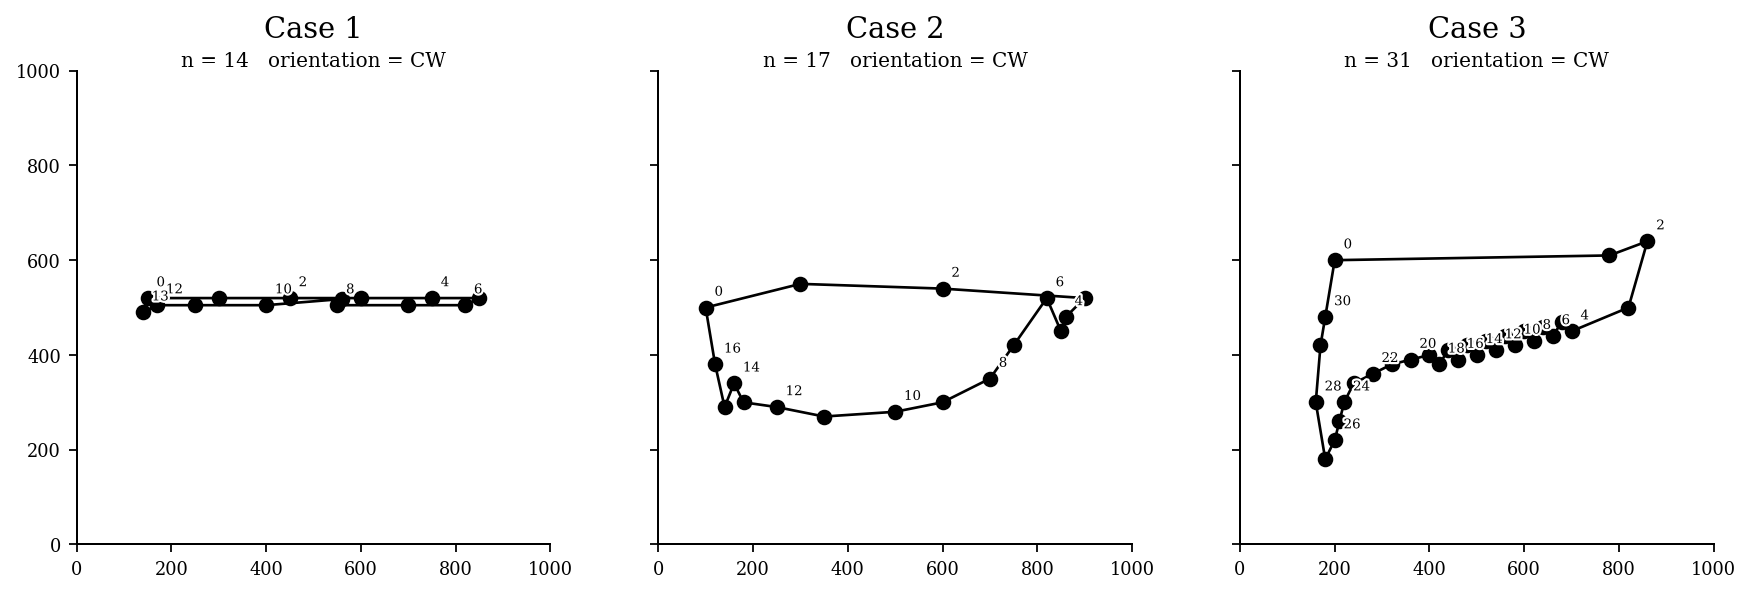
\includegraphics[width=0.9\linewidth]{Pictures/polygon_cases.png}
    \caption{Visualization of the three representative polygon cases used in testing Melkman’s algorithm. 
    Case~1: collinear band with near-degenerate contact; 
    Case~2: dual-pocket polygon; 
    Case~3: interior-point skipping with sparse expansion.}
\end{figure}

\textbf{Summary of coverage:}
The three designed cases jointly encompass the major geometric and numerical challenges identified in Section~3.1. 
Case~1 focuses on numerical stability under collinearity, near-degenerate geometry, and near-contact configurations, verifying that orientation, convexity, and initialization logic remain robust at precision limits. 
Case~2 targets the algorithm’s structural correctness during hull updates by introducing concave pockets that activate both front and back deque operations, testing update order and boundary integrity. 
Case~3 evaluates performance and correctness in mixed-density inputs, where numerous interior points are interleaved with sparse exterior ones, validating the skip logic and maintenance of linear-time behavior.

Together, these cases comprehensively test Melkman’s algorithm across initialization, inside-testing, and deque-update phases. 
They confirm that the implementation is robust to collinearity, concavity, and numerical perturbation, while preserving correctness and $\mathcal{O}(n)$ efficiency across all representative polygon configurations.

\subsection*{4. Visualization and Results Analysis}\

Following the design principles and definitions described in previous sections, the Melkman convex hull algorithm was implemented and tested on the three representative polygon cases defined in Section~3. 
The results are shown in Figure~\ref{fig:hulls}, where each subfigure corresponds to one of the test cases: 
Case~1 (collinear band with near-degenerate contact), 
Case~2 (dual-pocket polygon), 
and Case~3 (interior-point skipping and sparse expansion).

\begin{figure}[H]
    \centering
    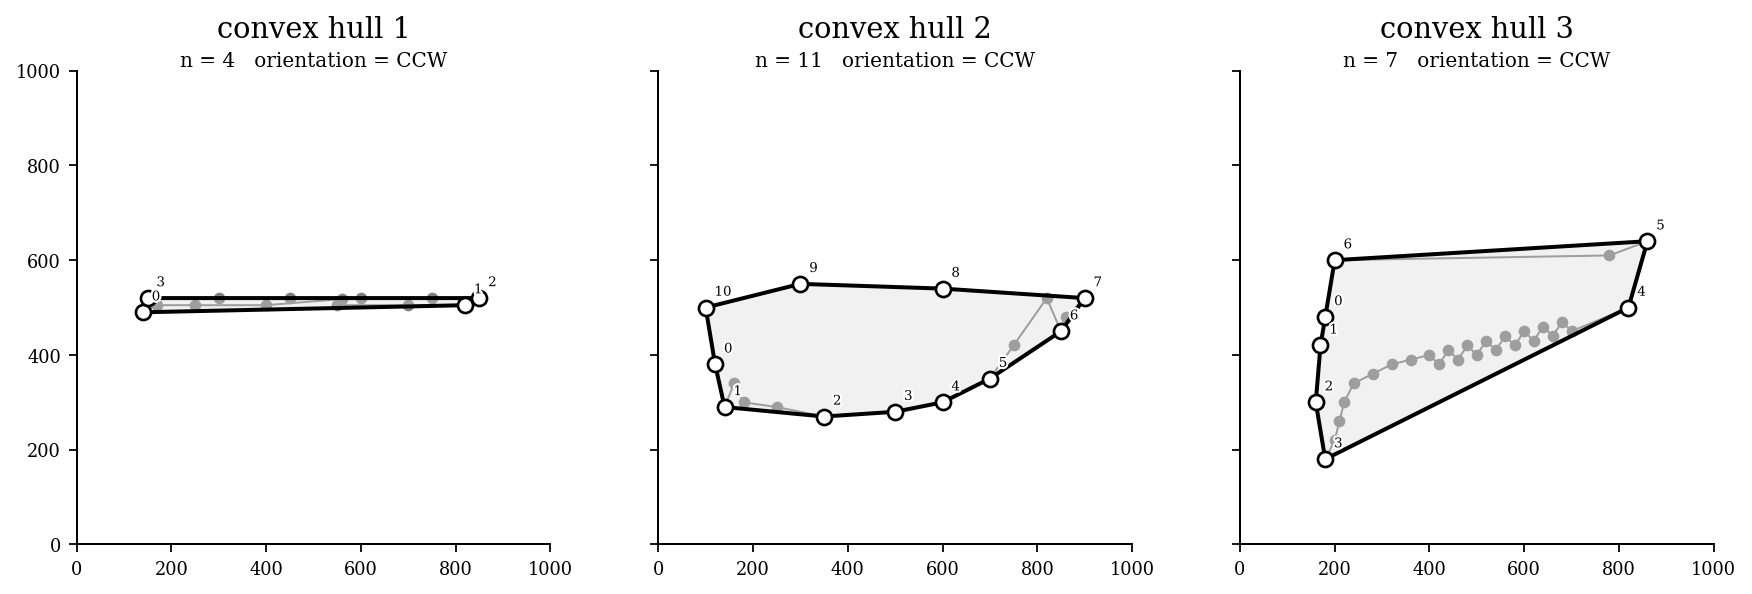
\includegraphics[width=0.95\linewidth]{Pictures/hulls.png}
    \caption{Visualization of convex hull results for the three designed test cases. 
    Each subfigure shows the original polygon (gray line and points) and the computed convex hull (bold black outline). 
    Hull vertices are labeled in counterclockwise order, and $n$ denotes the number of vertices in each polygon.}
    \label{fig:hulls}
\end{figure}

\textbf{Result correctness and analysis:}  
The visual outcomes confirm that Melkman’s algorithm produces the expected convex boundaries for all three input categories.

For \emph{Case~1}, only the extreme vertices of the upper and lower collinear bands are retained, while all intermediate collinear points are correctly excluded from the hull. 
The narrow-band configuration demonstrates stable orientation evaluation even when $\text{orient}(a,b,c) \approx 0$, indicating numerical robustness against near-degenerate geometry.

For \emph{Case~2}, the presence of two concave pockets successfully triggers deque updates at both ends. 
The hull reconstruction after each concave indentation preserves convexity and counterclockwise orientation, verifying the correctness of the bidirectional popping mechanism.

For \emph{Case~3}, the majority of interior points are efficiently skipped, while a few exterior vertices correctly expand the hull boundary. 
The algorithm maintains linear-time behavior since each vertex is processed at most once, confirming that the skip logic prevents redundant operations.

Overall, the visualization results align perfectly with the theoretical expectations. 
Melkman’s algorithm demonstrates robustness across numerical edge cases, correctness in deque-based updates. 
The generated convex hulls exhibit clean, non-intersecting boundaries that accurately enclose the input polygons.

\subsection*{5. Time Complexity Analysis}\

\paragraph{5.1 Theoretical}\

Melkman’s algorithm achieves linear-time complexity $\mathcal{O}(n)$ with respect to the number of vertices in the input polygon. 
The efficiency arises from its incremental and deterministic construction process, which guarantees that each vertex is handled a constant number of times. 

During the main loop, each vertex $p_i$ is read exactly once in the scanning order of the polygon. 
For each $p_i$, the algorithm performs a constant number of orientation tests and at most a few deque operations. 
Each vertex can be inserted into and removed from the deque at most once per end—once when it enters the convex hull and once when it is later popped due to a non-left turn. 
Therefore, the total number of deque operations over the entire run is proportional to $n$.

The orientation test $\text{orient}(a,b,c)$, which involves a few arithmetic operations on vertex coordinates, also executes $\mathcal{O}(1)$ per call. 
Even under degenerate cases such as long collinear sequences, each vertex still contributes only a bounded number of constant-time comparisons before either being skipped or becoming part of the hull.

As a result, the total computational cost can be expressed as:
\[
T(n) = c_1 n + c_2 n + c_3 n = \mathcal{O}(n),
\]
where $c_1$, $c_2$, and $c_3$ correspond to the constant-time costs of orientation evaluation, deque maintenance, and inside-testing respectively. 
No nested loops dependent on $n$ exist in the algorithm, and no vertex is ever revisited or reprocessed after being finalized in the hull. 

Hence, Melkman’s convex hull algorithm is theoretically proven to run in $\mathcal{O}(n)$ time for any simple polygon input, achieving optimal performance for this class of problems.

\paragraph{5.2 Empirical}\

To validate the theoretical time complexity, an experimental evaluation was conducted using a series of polygons with progressively increasing vertex counts. 
Nine polygon sets were generated to provide a controlled range of input sizes, ensuring both reproducibility and consistent geometric diversity. 
The generated polygons are visualized in Figure~\ref{fig:testpolys}, and their corresponding convex hulls, computed using the implemented Melkman algorithm, are shown in Figure~\ref{fig:testhulls}. 
Each convex hull result was visually verified to confirm correctness before performing timing and operation-count measurements.

\begin{figure}[H]
    \centering
    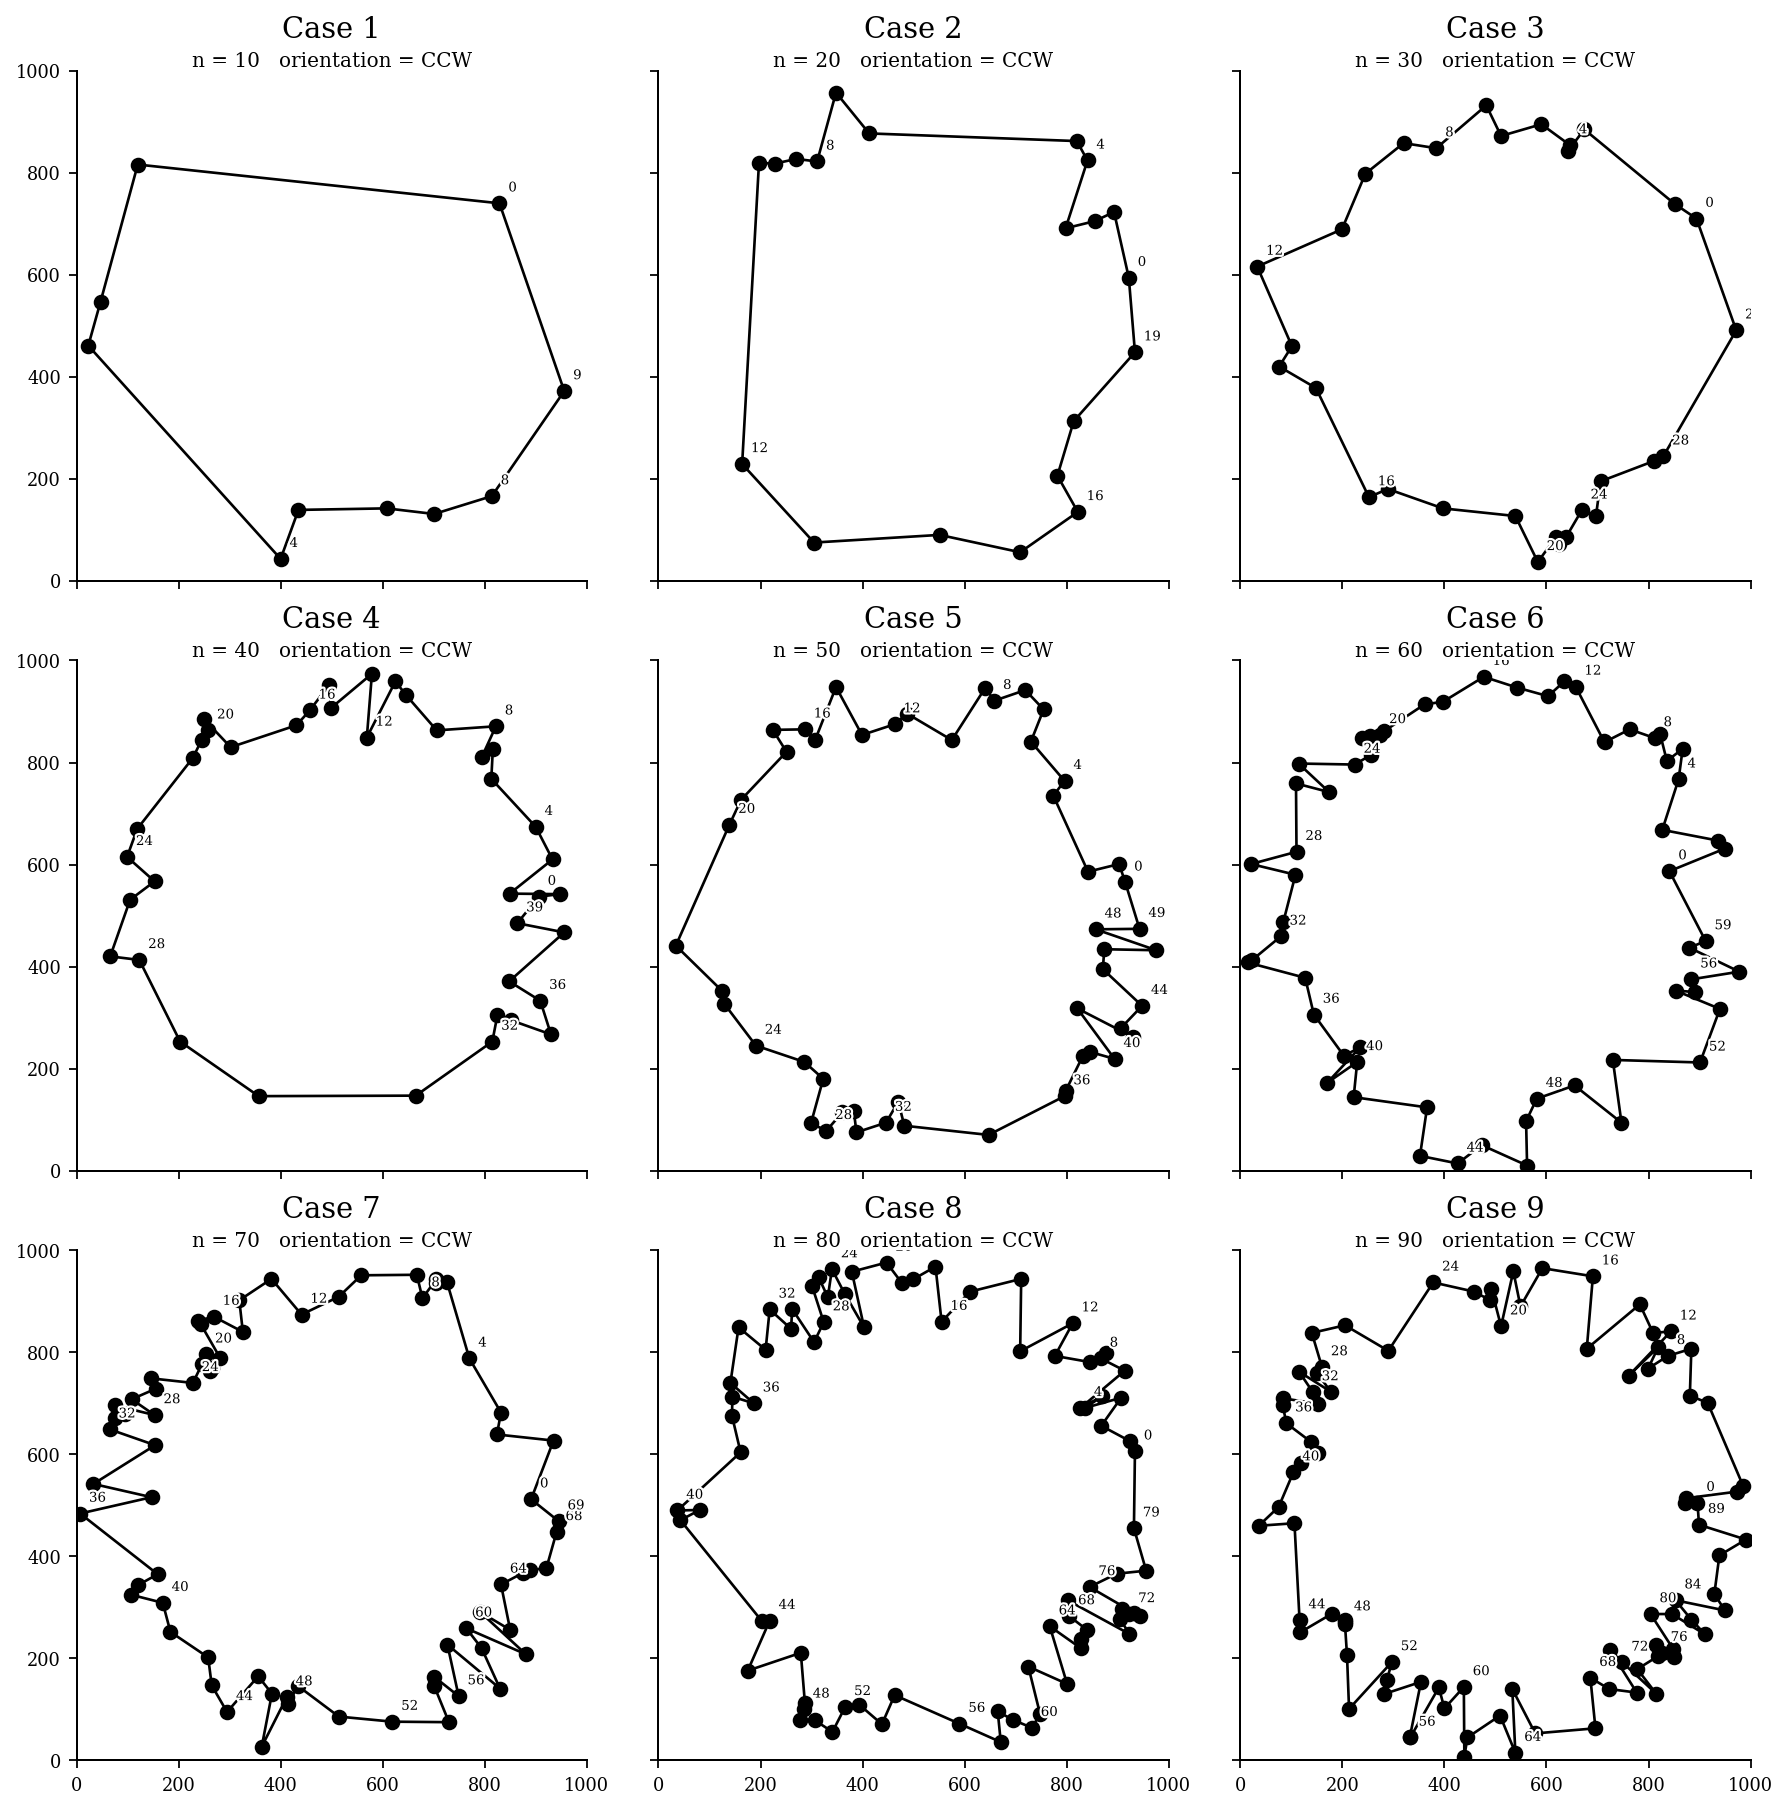
\includegraphics[width=0.95\linewidth]{Pictures/test_polygon_cases.png}
    \caption{Generated simple polygon test cases with increasing vertex counts ($n=10$ to $n=90$). 
    Each subfigure represents a distinct input size used for empirical complexity evaluation.}
    \label{fig:testpolys}
\end{figure}

\begin{figure}[H]
    \centering
    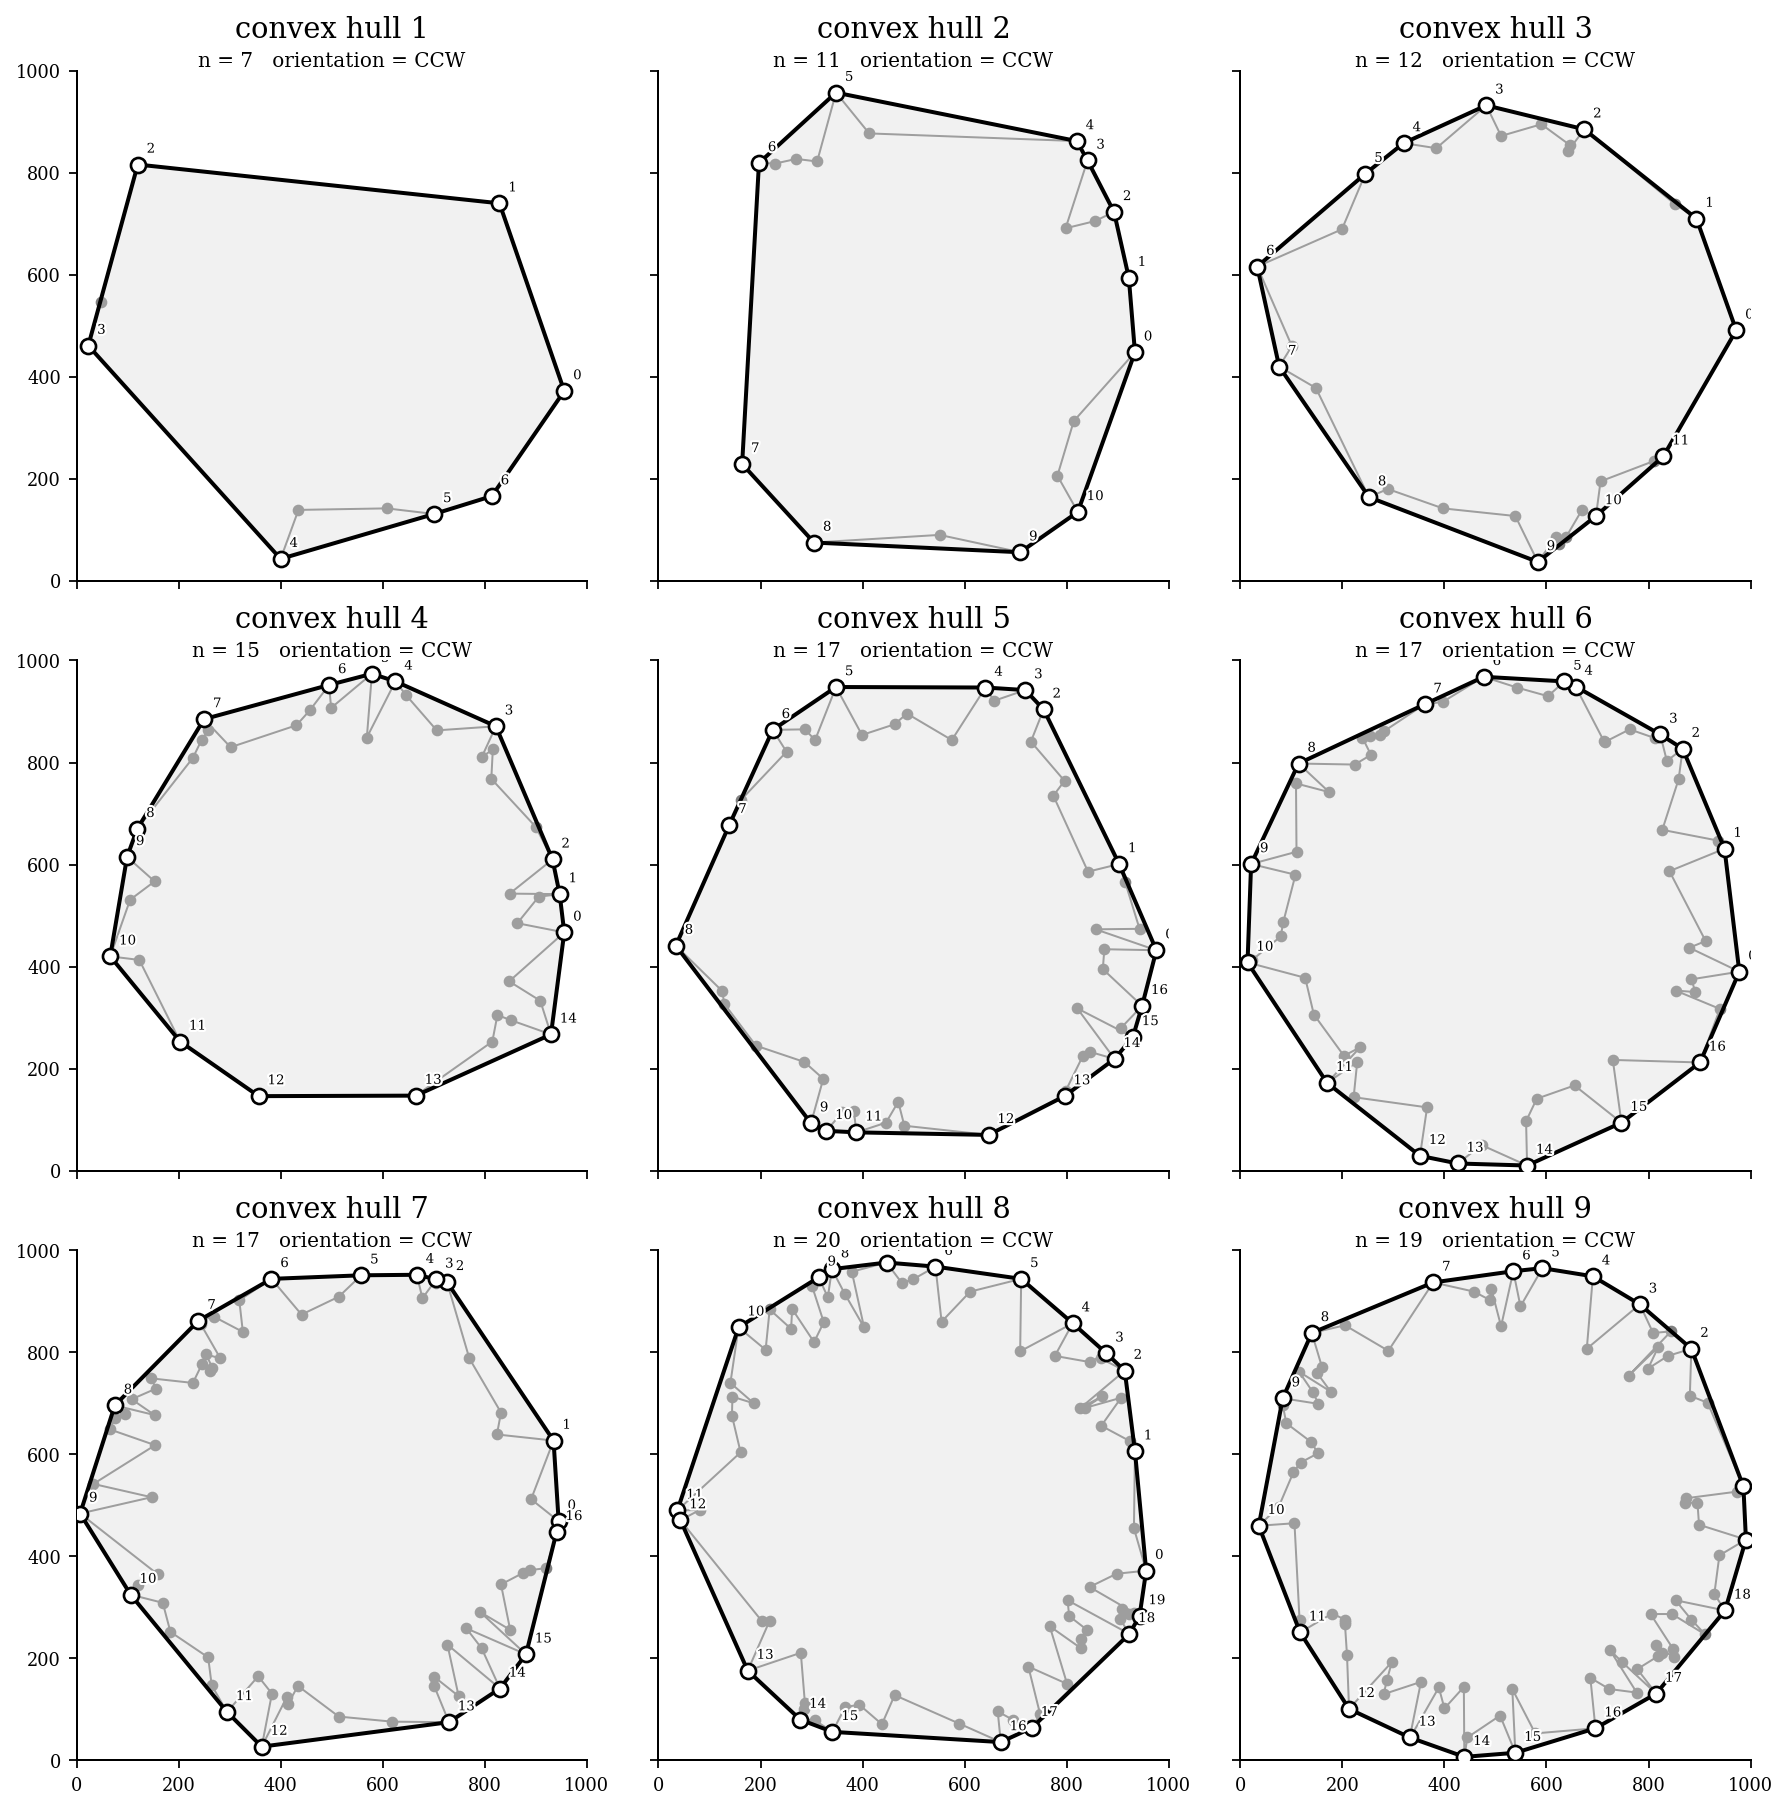
\includegraphics[width=0.95\linewidth]{Pictures/test_hulls.png}
    \caption{Convex hulls computed by Melkman’s algorithm for the test polygons shown in Figure~\ref{fig:testpolys}. 
    The results confirm correctness and stability across all polygon sizes.}
    \label{fig:testhulls}
\end{figure}

After correctness verification, execution time and total operation counts (including orientation, cross-product, and deque operations) were recorded for each test size. 
The results were then fitted to linear and power-law models, as shown in Figure~\ref{fig:complexity}.

\begin{figure}[H]
    \centering
    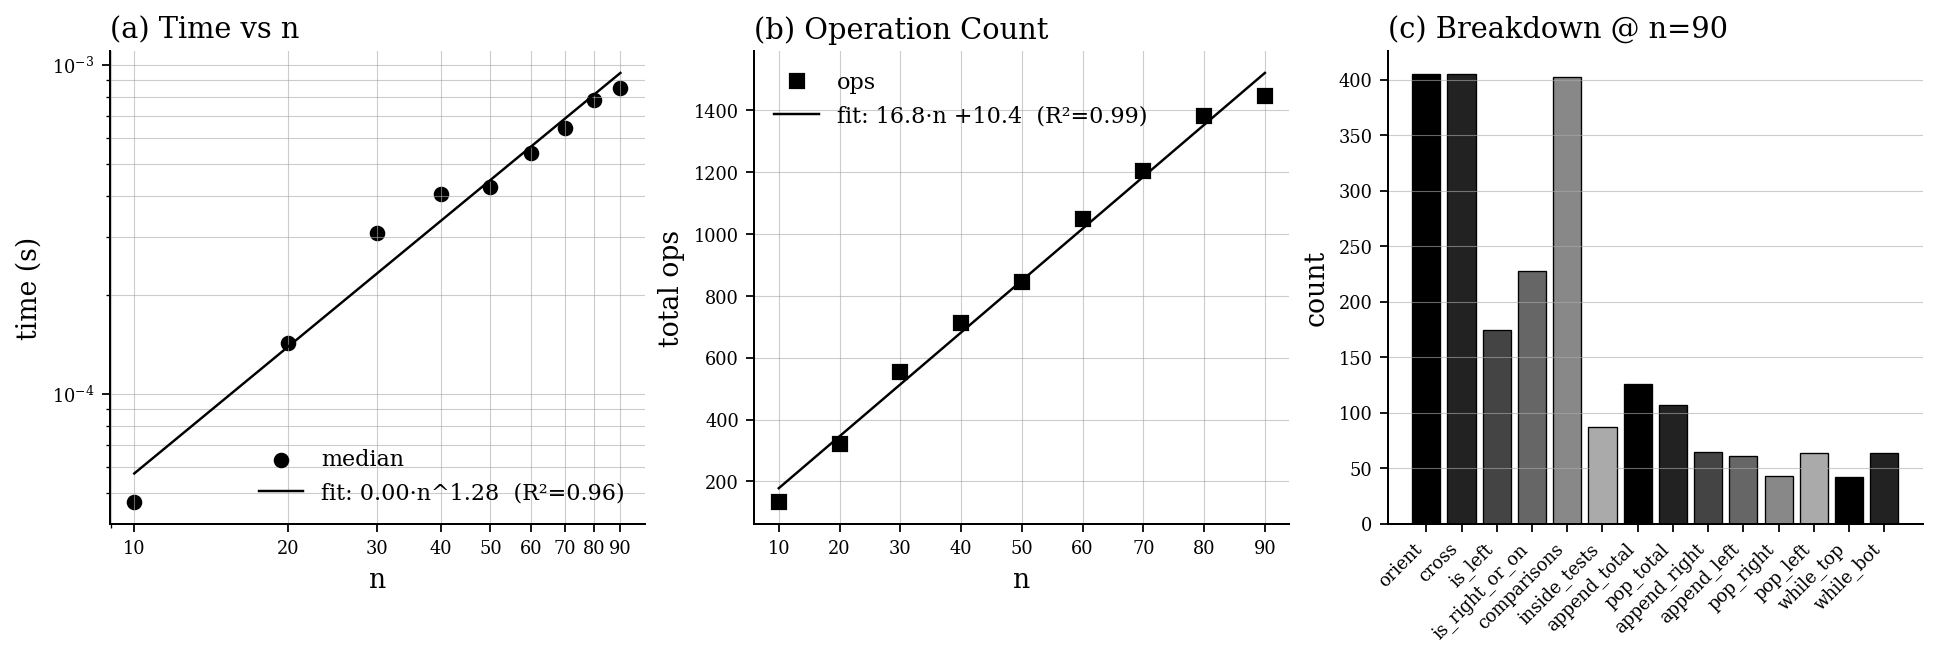
\includegraphics[width=0.95\linewidth]{Pictures/melkman_complexity.png}
    \caption{Empirical complexity analysis of Melkman’s algorithm. 
    (a) Median runtime versus input size $n$, fitted with $T(n)\propto n^{1.28}$ ($R^2=0.96$); 
    (b) total operation count showing a nearly perfect linear fit ($R^2=0.99$); 
    (c) operation breakdown at $n=90$, indicating that orientation and cross-product computations dominate total cost.}
    \label{fig:complexity}
\end{figure}

\textbf{Discussion:}
The measured runtime exhibits an almost linear growth with respect to the number of vertices, with an empirical fit of approximately $T(n)\!\propto\!n^{1.28}$, closely matching the theoretical $\mathcal{O}(n)$ expectation. 
The total operation count maintains a strictly linear relationship with $n$, confirming that each vertex contributes only a constant number of geometric and deque operations. 
The operation breakdown further shows that the majority of computational effort comes from orientation and cross-product evaluations, while deque operations remain minimal.

Overall, the empirical data strongly supports the theoretical claim that Melkman’s convex hull algorithm operates in linear time $\mathcal{O}(n)$, achieving both correctness and computational efficiency across varying input sizes.


\newpage
\problem{General Voronoi Diagram (Power Diagram Variant)}

Study general Voronoi diagrams and implement one variant of your choice.\bigskip

\noindent \textbf{Reference:} Slides of General Voronoi.

\noindent \textbf{Requirements:}
\begin{enumerate}
    \item Explain which variant you chose and why.
    \item Implement the algorithm with proper data structures.
    \item Visualize the result (2D plot showing the sites and Voronoi regions).
    \item Analyze the time and space complexity.
    \item Test cases with at least three different point configurations.
\end{enumerate}

\newpage

\subsection*{1. Variant Selection and Motivation}

The variant selected in this study is the \textbf{Power Diagram} (also known as the Laguerre–Voronoi Diagram), due to its strong theoretical and practical relevance to my ongoing research on three-dimensional medical image reconstruction.  
In 3D ultrasound image segmentation and reconstruction, it is often necessary to partition the space into weighted regions according to the spatial features or importance of different points, in order to generate structurally consistent and geometrically continuous volumetric representations.  
By introducing additive weights into the distance metric, the Power Diagram allows each cell to depend not only on spatial position but also on local weighting factors, which aligns well with the inherently non-uniform distribution of anatomical structures in medical images.  
Its convexity and controllability ensure numerical stability in geometric computations, while its formulation naturally extends to three dimensions and connects seamlessly with Delaunay triangulation and regular tessellation methods.  
Therefore, the Power Diagram provides both a solid theoretical foundation and a practical geometric framework for understanding and implementing weighted spatial partitioning in 3D medical image reconstruction.

\subsection*{2. Problem Definition and Notation}

\textbf{Input.}  
A finite set of weighted sites
\[
S=\{(x_i,y_i,w_i)\mid i=1,\dots,n\}\subset\mathbb{R}^2\times\mathbb{R},
\]
where $(x_i,y_i)$ is the location of site $s_i$ and $w_i$ is a scalar weight controlling its influence.

\textbf{Power distance.}  
For $p=(x,y)\in\mathbb{R}^2$ and $s_i=(x_i,y_i,w_i)$,
\[
\phi_i(p)=\|p-s_i\|^2-w_i .
\]
This definition yields affine bisectors between any pair of sites.

\textbf{Power cell.}  
The cell of $s_i$ is
\[
V_i=\{p\in\mathbb{R}^2\mid \phi_i(p)\le \phi_j(p),\ \forall j\neq i\},
\]
i.e., the intersection of half-planes that favor $s_i$ over every $s_j$.

\textbf{Output.}  
A per-site list of half-planes encoding the diagram rather than explicit polygon vertices.  
For each $s_i$,
\[
\mathcal{H}_i=\{(a_{ij},b_{ij},c_{ij})\mid a_{ij}x+b_{ij}y\le c_{ij},\ j\neq i\},
\]
where each triple represents the kept side of the bisector $\phi_i\le\phi_j$.  
Cells are implicit as $V_i=\bigcap_{H\in\mathcal{H}_i}H$.  
With \texttt{stats=True}, the procedure returns operation counts and the asymptotic summary $\Theta(n^2)$ for time and space.

\textbf{Goal.}  
Construct the per-site half-plane sets $\{\mathcal{H}_i\}$ for a Power Diagram, visualize resulting cells by clipping over a bounding box when needed, and analyze theoretical and empirical complexity.

\textbf{Notations.}  
\begin{itemize}
  \item $s_i=(x_i,y_i,w_i)$: the $i$-th weighted site.
  \item $\phi_i(p)$: power distance from $p$ to $s_i$.
  \item $V_i$: implicit cell of $s_i$ given by $\bigcap \mathcal{H}_i$.
  \item $(a,b,c)$: half-plane coefficients for $ax+by\le c$.
  \item $B=[x_{\min},y_{\min},x_{\max},y_{\max}]$: rendering/clipping box used only for visualization.
  \item $H_{ij}$: the half-plane $\{p\mid \phi_i(p)\le \phi_j(p)\}$ contributing one $(a_{ij},b_{ij},c_{ij})$ to $\mathcal{H}_i$.
\end{itemize}

\subsection*{3. Data Structures and Algorithm}

\paragraph{3.1 Data Structures}\

\begin{itemize}
    \item \textbf{Site list:}  
    A sequential array \texttt{sites\_in[i] = (x, y, w)} storing the integer coordinates and weights of all input sites.  
    Each element corresponds to a weighted site $s_i = (x_i, y_i, w_i)$ used to generate one power cell.

    \item \textbf{Half-plane representation:}  
    For every ordered pair of distinct sites $(s_i, s_j)$, the bisector of the power distance equation $\phi_i(p)=\phi_j(p)$
    can be written as a linear inequality
    \[
    a_{ij}x + b_{ij}y \le c_{ij},
    \]
    where 
    \[
    a_{ij} = 2(x_j - x_i), \quad
    b_{ij} = 2(y_j - y_i), \quad
    c_{ij} = (x_j^2 + y_j^2) - (x_i^2 + y_i^2) + (w_i - w_j).
    \]
    Each tuple $(a,b,c)$ is stored as a \texttt{HalfPlane} record satisfying the form \texttt{ax + by <= c}.  
    All half-planes associated with one site are grouped as
    \[
    \mathcal{H}_i = \{(a_{ij}, b_{ij}, c_{ij}) \mid j \ne i\},
    \]
    representing the complete intersection that defines $V_i$.

    \item \textbf{Per-site region list:}  
    A list of lists \texttt{power\_regions[i]} that stores $\mathcal{H}_i$ for each site.  
    This structure provides constant-time access to all bounding half-planes of any cell and supports later polygon reconstruction through half-plane clipping.

    \end{itemize}

\paragraph{3.2 Algorithmic Overview}\

The procedure constructs the Power Diagram by enumerating all ordered site pairs, deriving the affine half-planes that favor each site, and grouping these half-planes per site. Given a weighted set \(S=\{(x_i,y_i,w_i)\}_{i=1}^n\) with \(n\ge 2\), the algorithm initializes an empty container for each site’s constraints \(\mathcal H_i\). For every \(j\neq i\), it computes the coefficients of the bisector \(\phi_i(p)\le \phi_j(p)\) in the linear form \(a_{ij}x+b_{ij}y\le c_{ij}\) using
\[
a_{ij}=2(x_j-x_i),\qquad
b_{ij}=2(y_j-y_i),\qquad
c_{ij}=(x_j^2+y_j^2)-(x_i^2+y_i^2)+(w_i-w_j).
\]
The triple \((a_{ij},b_{ij},c_{ij})\) is appended to \(\mathcal H_i\). After processing all pairs, the output is the collection \(\{\mathcal H_i\}_{i=1}^n\). Polygonal cells \(V_i\) can be recovered later by clipping \(\bigcap_{H\in\mathcal H_i}H\) against a rendering bounding box. 
\begin{algorithm}[H]
\caption{BUILD\_POWER\_CELLS}
\begin{algorithmic}[1]
\Require Sites \(S=\{(x_i,y_i,w_i)\}_{i=1}^n\) with \(n\ge 2\)
\Ensure Per-site half-plane sets \(\{\mathcal H_i\}_{i=1}^n\)

\State \( \text{PowerRegions} \leftarrow [\,]\)
\For{\(i \gets 1 \ \textbf{to}\ n\)}
    \State \( \mathcal H_i \leftarrow [\,]\); \( (x_i,y_i,w_i) \leftarrow S[i]\)
    \For{\(j \gets 1 \ \textbf{to}\ n\)}
        \If{\(j = i\)} \State \textbf{continue} \EndIf
        \State \( (x_j,y_j,w_j) \leftarrow S[j]\)
        \State \( a \leftarrow 2(x_j-x_i),\quad b \leftarrow 2(y_j-y_i)\)
        \State \( c \leftarrow (x_j^2+y_j^2)-(x_i^2+y_i^2)+(w_i-w_j)\)
        \State append \((a,b,c)\) to \(\mathcal H_i\)
    \EndFor
    \State append \(\mathcal H_i\) to \(\text{PowerRegions}\)
\EndFor
\State \Return \(\text{PowerRegions}\)
\end{algorithmic}
\end{algorithm}

Each clipping preserves convexity, and the total set of cells forms a complete partition of the plane.

\subsection*{4. Test Case Design}

\paragraph{4.1 Special Cases}\

In the Power Diagram construction, several degenerate and numerically sensitive configurations may arise due to the interaction between spatial distribution and weight magnitude.  
Unlike the standard Voronoi diagram, where only geometric proximity determines cell boundaries, the weighted form introduces additional conditions that can lead to cell suppression, unbounded regions, or numerical instability.  
To ensure robustness and completeness of the implementation, representative special cases are designed to cover the following scenarios:

\begin{itemize}
    \item \textbf{Extremely weighted dominance.}  
    When one site has a substantially larger weight than all others, its corresponding cell can expand disproportionately, possibly eliminating or minimizing neighboring cells.  
    This case tests whether the algorithm correctly handles \emph{empty cells} (sites whose feasible half-plane intersection vanishes) without numerical breakdown.

    \item \textbf{Unweighted baseline (degeneration to standard Voronoi).}  
    Setting all weights to zero reduces the formulation to the classical Voronoi diagram, in which all bisectors are unbiased Euclidean midlines.  
    This baseline verifies the consistency of half-plane generation and correctness of affine bisector computation under the unweighted limit.

    \item \textbf{Collinear or nearly collinear sites.}  
    When multiple sites are placed on the same straight line, the resulting bisectors may intersect in unstable or near-parallel configurations.  
    Such cases produce long, narrow, or even semi-infinite cells.  
    They test the stability of orientation and clipping logic under limited angular diversity.

    \item \textbf{Negative weights.}  
    Negative weights correspond to virtual “imaginary circles” in the power distance formulation.  
    Although geometrically valid, they invert the direction of certain half-planes and may enlarge cells unexpectedly.  
    This scenario ensures that the implementation remains correct for all real-valued weights and that sign changes do not disrupt linear partitioning.

    \item \textbf{Coincident sites (identical coordinates with different weights).}  
    When two or more sites share the same spatial position but possess different weights, the cell of the lower-weight site should vanish completely.  
    This case examines whether the algorithm correctly distinguishes dominance in the power comparison and properly identifies zero-area cells.

\end{itemize}

Together, these special cases comprehensively test the geometric and numerical stability of the Power Diagram implementation.  
They ensure that the algorithm remains valid across extreme weight differences, degeneracy to the classical Voronoi case, collinearity-induced instability, negative-weight configurations, and coincident-site dominance, all of which are critical for achieving robustness in both two-dimensional analysis and potential three-dimensional extensions.
\paragraph{4.2 Case 1: Unweighted Baseline with Collinear Strip Degeneracy}\

\textbf{Objectives and algorithmic checks:}
\begin{enumerate}
    \item Verify degeneration to the classical Voronoi diagram when all weights vanish ($w_i\equiv 0$); confirm that affine bisectors are computed correctly from the power-distance formulation.
    \item Assess numerical stability under extended collinearity: multiple sites placed on a common line produce near-parallel bisectors and elongated cells; check that half-plane generation and later polygon recovery remain consistent.
    \item Ensure no spurious empty cells arise in the unweighted regime; validate that all cells are bounded or unbounded as predicted by geometry rather than numerical artifacts.
\end{enumerate}

\textbf{Construction method:}
Ten sites are used with $w_i=0$ for all $i$. Five sites are placed on a single line to induce collinearity, e.g., along $y=520$ at $x\in\{160, 320, 500, 680, 840\}$. The remaining five are scattered off the line to prevent an overall 1D collapse, e.g., $(200,260)$, $(780,610)$, $(880,640)$, $(180,180)$, $(420,360)$. This layout yields a pronounced “collinear strip” interacting with a sparse off-line background, forcing near-parallel bisectors and long faces while preserving a genuinely 2D configuration.

\textbf{Conclusion:}
Case~1 isolates two critical aspects in a controlled setting: the $w_i=0$ limit, which must reproduce standard Voronoi behavior, and the sensitivity of affine bisectors under collinearity. It provides a clean baseline to confirm correct bisector construction from the power model and to test stability when sites induce narrow or semi-infinite cells, while avoiding empty-cell artifacts expected only under extreme weighting.

\paragraph{4.3 Case 2: Extreme Weight Dominance with a Negative-Weight Outlier}\

\textbf{Objectives and algorithmic checks:}
\begin{enumerate}
    \item Validate dominance under large positive weights: confirm that a single high-weight site expands its cell and can suppress neighbors, producing correctly detected \emph{empty cells} when the half-plane intersection vanishes.
    \item Verify sign handling for negative weights: ensure that the bisector orientation and the inequality side ($a_{ij}x+b_{ij}y\le c_{ij}$) remain correct when $w_j<0$, and that linear partitioning is preserved.
    \item Test numerical stability under weight-scale disparity: large $|w|$ must not flip half-planes due to round-off, and the resulting cells must remain geometrically consistent upon polygon recovery by clipping.
\end{enumerate}

\textbf{Construction method:}
Ten sites are placed with heterogeneous weights. One site at the scene center (e.g., $(520,520)$) is assigned a very large weight $w_c\!\gg\!0$. Around it, seven to eight sites are positioned in a loose ring spanning all quadrants with medium or small weights to induce compression. A remote outlier site (e.g., $(940,220)$) is given a \emph{negative} weight $w_{-}\!<\!0$ to exercise sign-sensitive bisector formation. All coordinates are chosen to avoid exact symmetry, preventing accidental cancellations in the affine coefficients.

\textbf{Conclusion:}
Case~2 targets two weighted-specific edge conditions absent in classical Voronoi: global dominance induced by extreme positive weights and correctness under negative weights. It stresses the half-plane construction $a_{ij},b_{ij},c_{ij}$ with large-magnitude $(w_i-w_j)$, checks that suppressed neighbors are reported as empty cells, and confirms that linear bisectors and cell topology remain valid across strong weight contrasts.

\paragraph{4.4 Case 3: Coincident Sites with Mild Weights and a Weak Collinear Triplet}\

\textbf{Objectives and algorithmic checks:}
\begin{enumerate}
    \item Validate power-based dominance at identical coordinates: when two sites share the same position, confirm that the higher-weight site fully owns the location and the lower-weight site degenerates to a zero-area (empty) cell.
    \item Test local stability with a short collinear segment: three nearly aligned sites should yield elongated but well-formed affine edges without topological artifacts during polygon recovery.
    \item Ensure absence of unintended global swallowing: with mild weights elsewhere, non-coincident sites should retain regular cells; verify correct half-plane orientation and boundedness where expected.
\end{enumerate}

\textbf{Construction method:}
Ten sites are used with moderate weight variation. Two \emph{coincident pairs} are created at two distinct coordinates, e.g., $q_1=(360,420)$ and $q_2=(720,380)$, with weights $w^\text{hi}>w^\text{lo}$ at each location to enforce dominance and degeneracy. The remaining six sites are scattered to form a generic background with small-to-medium weights. Among these six, choose three to form a \emph{weak collinear} triplet spanning a short segment (e.g., $(260,520)$, $(310,515)$, $(360,510)$), avoiding long-range alignment that could collapse the diagram. Coordinates are selected to break symmetry and prevent accidental equalities in $a_{ij},b_{ij},c_{ij}$.

\textbf{Conclusion:}
Case~3 simultaneously exercises coincident-site dominance (zero-area detection), local collinearity robustness, and routine weighted behavior in the surrounding field. It confirms that the half-plane system correctly encodes priority at identical coordinates, produces stable affine bisectors near short collinear runs, and maintains clear topology without spurious empty cells beyond the intended degenerate pair.

\paragraph{4.5 Visual Summary and Case Coverage}\

\begin{figure}[H]
    \centering
    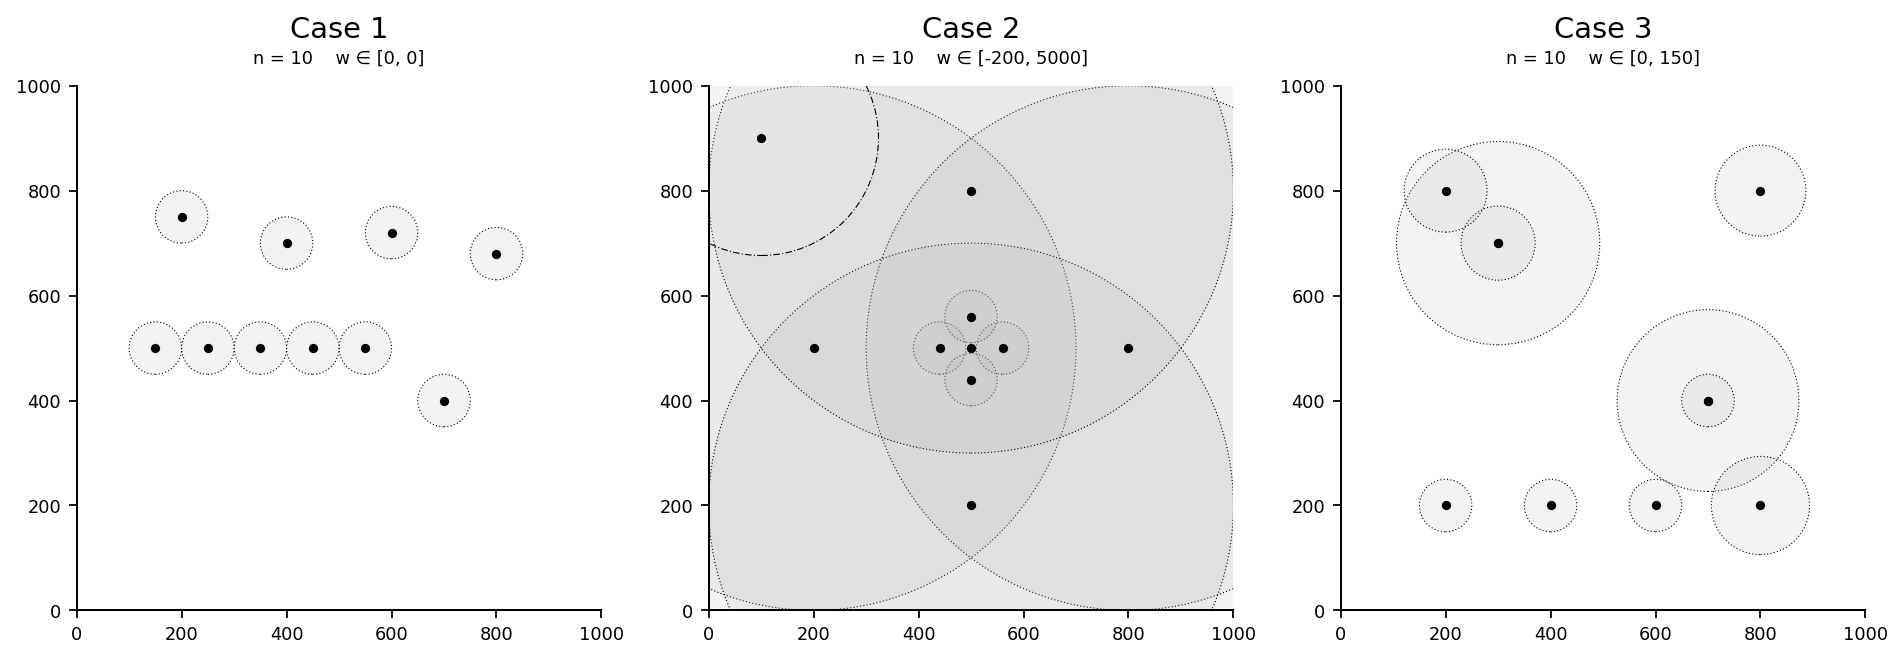
\includegraphics[width=0.95\linewidth]{Pictures/sites_cases.png}
    \caption{Site distributions and indicative weight circles for the three designed Power-Diagram cases. 
    Left: Case~1 (unweighted baseline with a collinear strip); 
    Middle: Case~2 (extreme positive weight at center plus a negative-weight outlier); 
    Right: Case~3 (two coincident-site pairs with mild weights and a weak collinear triplet).}
\end{figure}

\textbf{Summary of coverage.}
The trio of cases spans the principal geometric and weighted degeneracies relevant to Power Diagrams. 
Case~1 validates the $w_i\!\equiv\!0$ limit against standard Voronoi behavior while stressing affine bisectors under extended collinearity. 
Case~2 probes weight-scale disparity, confirming dominance-induced suppression and correctness for negative weights without breaking linear partitioning. 
Case~3 exercises coincident-site priority and local collinearity, verifying zero-area detection and stable edge formation in routine weighted settings. 
Together, they provide a compact yet comprehensive stress test for half-plane generation, empty-cell identification, and subsequent polygon recovery by clipping.

\subsection*{5. Visualization and Results Analysis}

Following the data structures and algorithmic framework described in previous sections, the implemented Power Diagram generator was applied to the three representative test cases introduced in Section~4.  
The resulting diagrams are shown in Figure~\ref{fig:power_diagrams}, where each subfigure corresponds to one test case:
Case~1 (unweighted baseline with collinear strip),
Case~2 (extreme weight dominance with a negative-weight outlier),
and Case~3 (coincident-site pairs with mild weights and a weak collinear triplet).

\begin{figure}[H]
    \centering
    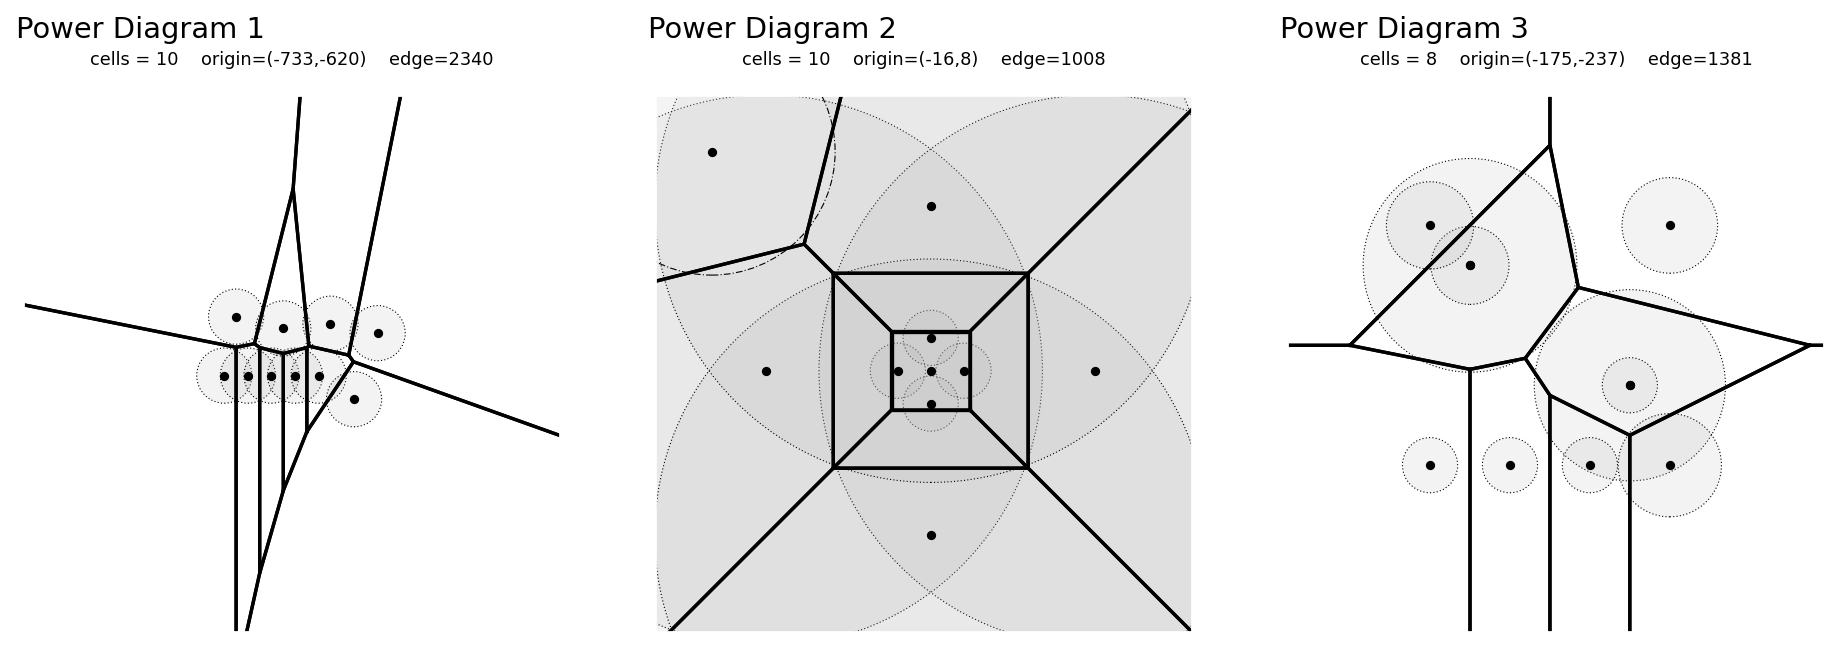
\includegraphics[width=0.95\linewidth]{Pictures/power_diagram.png}
    \caption{Visualization of Power Diagram results for the three designed test cases.
    Each subfigure shows the weighted sites (black dots) and their associated power cells (thick black lines). 
    Dashed circles indicate equivalent “power radii” $\sqrt{|w_i|}$ for visualization, and gray shading marks valid bounded cells.
    Case~1: $w_i\!\equiv\!0$ (standard Voronoi); 
    Case~2: strong central dominance with one negative-weight outlier; 
    Case~3: two coincident-site pairs and a weak collinear triplet.}
    \label{fig:power_diagrams}
\end{figure}

\textbf{Result correctness and analysis:}  
The visual outcomes confirm that the constructed half-plane system and subsequent clipping process correctly produce the expected linear partitions across all weighting regimes.

For \emph{Case~1}, the resulting diagram perfectly matches the standard Voronoi structure.  
All bisectors appear as straight Euclidean midlines, and the five collinear sites yield narrow or elongated regions without degeneracy.  
This confirms that the unweighted limit of the algorithm remains geometrically stable and numerically well-conditioned.

For \emph{Case~2}, the large central weight generates a dominant cell that expands across most of the domain, while several neighboring sites collapse into empty or near-zero cells, correctly reported as “swallowed” regions.  
The negative-weight outlier retains a valid and slightly enlarged cell, verifying that sign changes in $w_i$ are handled consistently and do not disrupt linearity or convexity of the cells.

For \emph{Case~3}, the coincident-site pairs behave as expected: the higher-weight site at each shared coordinate acquires a normal bounded region, whereas the lower-weight counterpart degenerates into a zero-area cell.  
The short collinear triplet produces locally parallel bisectors that remain numerically stable, confirming the robustness of half-plane intersection and clipping near near-degenerate alignments.

Overall, the visualization results align precisely with theoretical expectations.  
The Power Diagram implementation successfully handles unweighted, highly weighted, negative-weight, and coincident-site configurations using a unified half-plane formulation.  
All observed partitions are convex, non-overlapping, and exhibit clean boundaries, demonstrating both correctness and numerical stability of the proposed algorithm.

\subsection*{6. Complexity Analysis}

\paragraph{6.1 Theoretical}\

The Power Diagram construction algorithm operates by evaluating all ordered pairs of weighted sites and computing the affine half-plane coefficients for each interaction.  
Let \(n\) denote the number of sites in the input set \(S=\{(x_i,y_i,w_i)\}_{i=1}^n\).  
For each site \(s_i\), the algorithm iterates through all other sites \(s_j\ (j\neq i)\) to compute a bisector inequality of the form \(a_{ij}x+b_{ij}y\le c_{ij}\).  
This results in a total of \(n(n-1)\) half-plane equations generated across the entire set.

Each iteration involves a constant number of arithmetic operations—specifically, subtractions, multiplications, and additions—to derive the coefficients:
\[
a_{ij}=2(x_j-x_i),\quad b_{ij}=2(y_j-y_i),\quad
c_{ij}=(x_j^2+y_j^2)-(x_i^2+y_i^2)+(w_i-w_j).
\]
Since no iterative refinement, sorting, or geometric clipping occurs during this phase, every computation is performed in constant time.  
Therefore, the overall time complexity of the coefficient construction is:
\[
T(n) = c \cdot n(n-1) = \Theta(n^2),
\]
where \(c\) is a small constant representing the fixed arithmetic cost per bisector.

The space complexity is dominated by the storage of all half-plane triples \((a,b,c)\).  
Each site \(s_i\) maintains \((n-1)\) such records, giving a total storage requirement of:
\[
M(n) = n(n-1) = \Theta(n^2).
\]
Auxiliary memory for temporary variables and the output container is linear in \(n\), negligible compared to the quadratic term.

In summary:
\[
\text{Time complexity: } \Theta(n^2), \qquad
\text{Space complexity: } \Theta(n^2).
\]
This quadratic behavior is intrinsic to any naïve all-pairs construction of weighted bisectors, as every site-to-site relation must be evaluated once.  
Subsequent clipping against a bounding box, performed later for visualization, is linear in the number of half-planes per site and does not alter the overall asymptotic bound.

\paragraph{6.2 Empirical}\

To empirically validate the theoretical complexity derived in Section~6.1, two rounds of experiments were conducted using progressively larger site sets to observe time, operation, and memory scaling behavior.  
Each round generated multiple random site configurations with increasing $n$, ensuring statistical robustness and visual consistency across weighted distributions.

\begin{figure}[H]
    \centering
    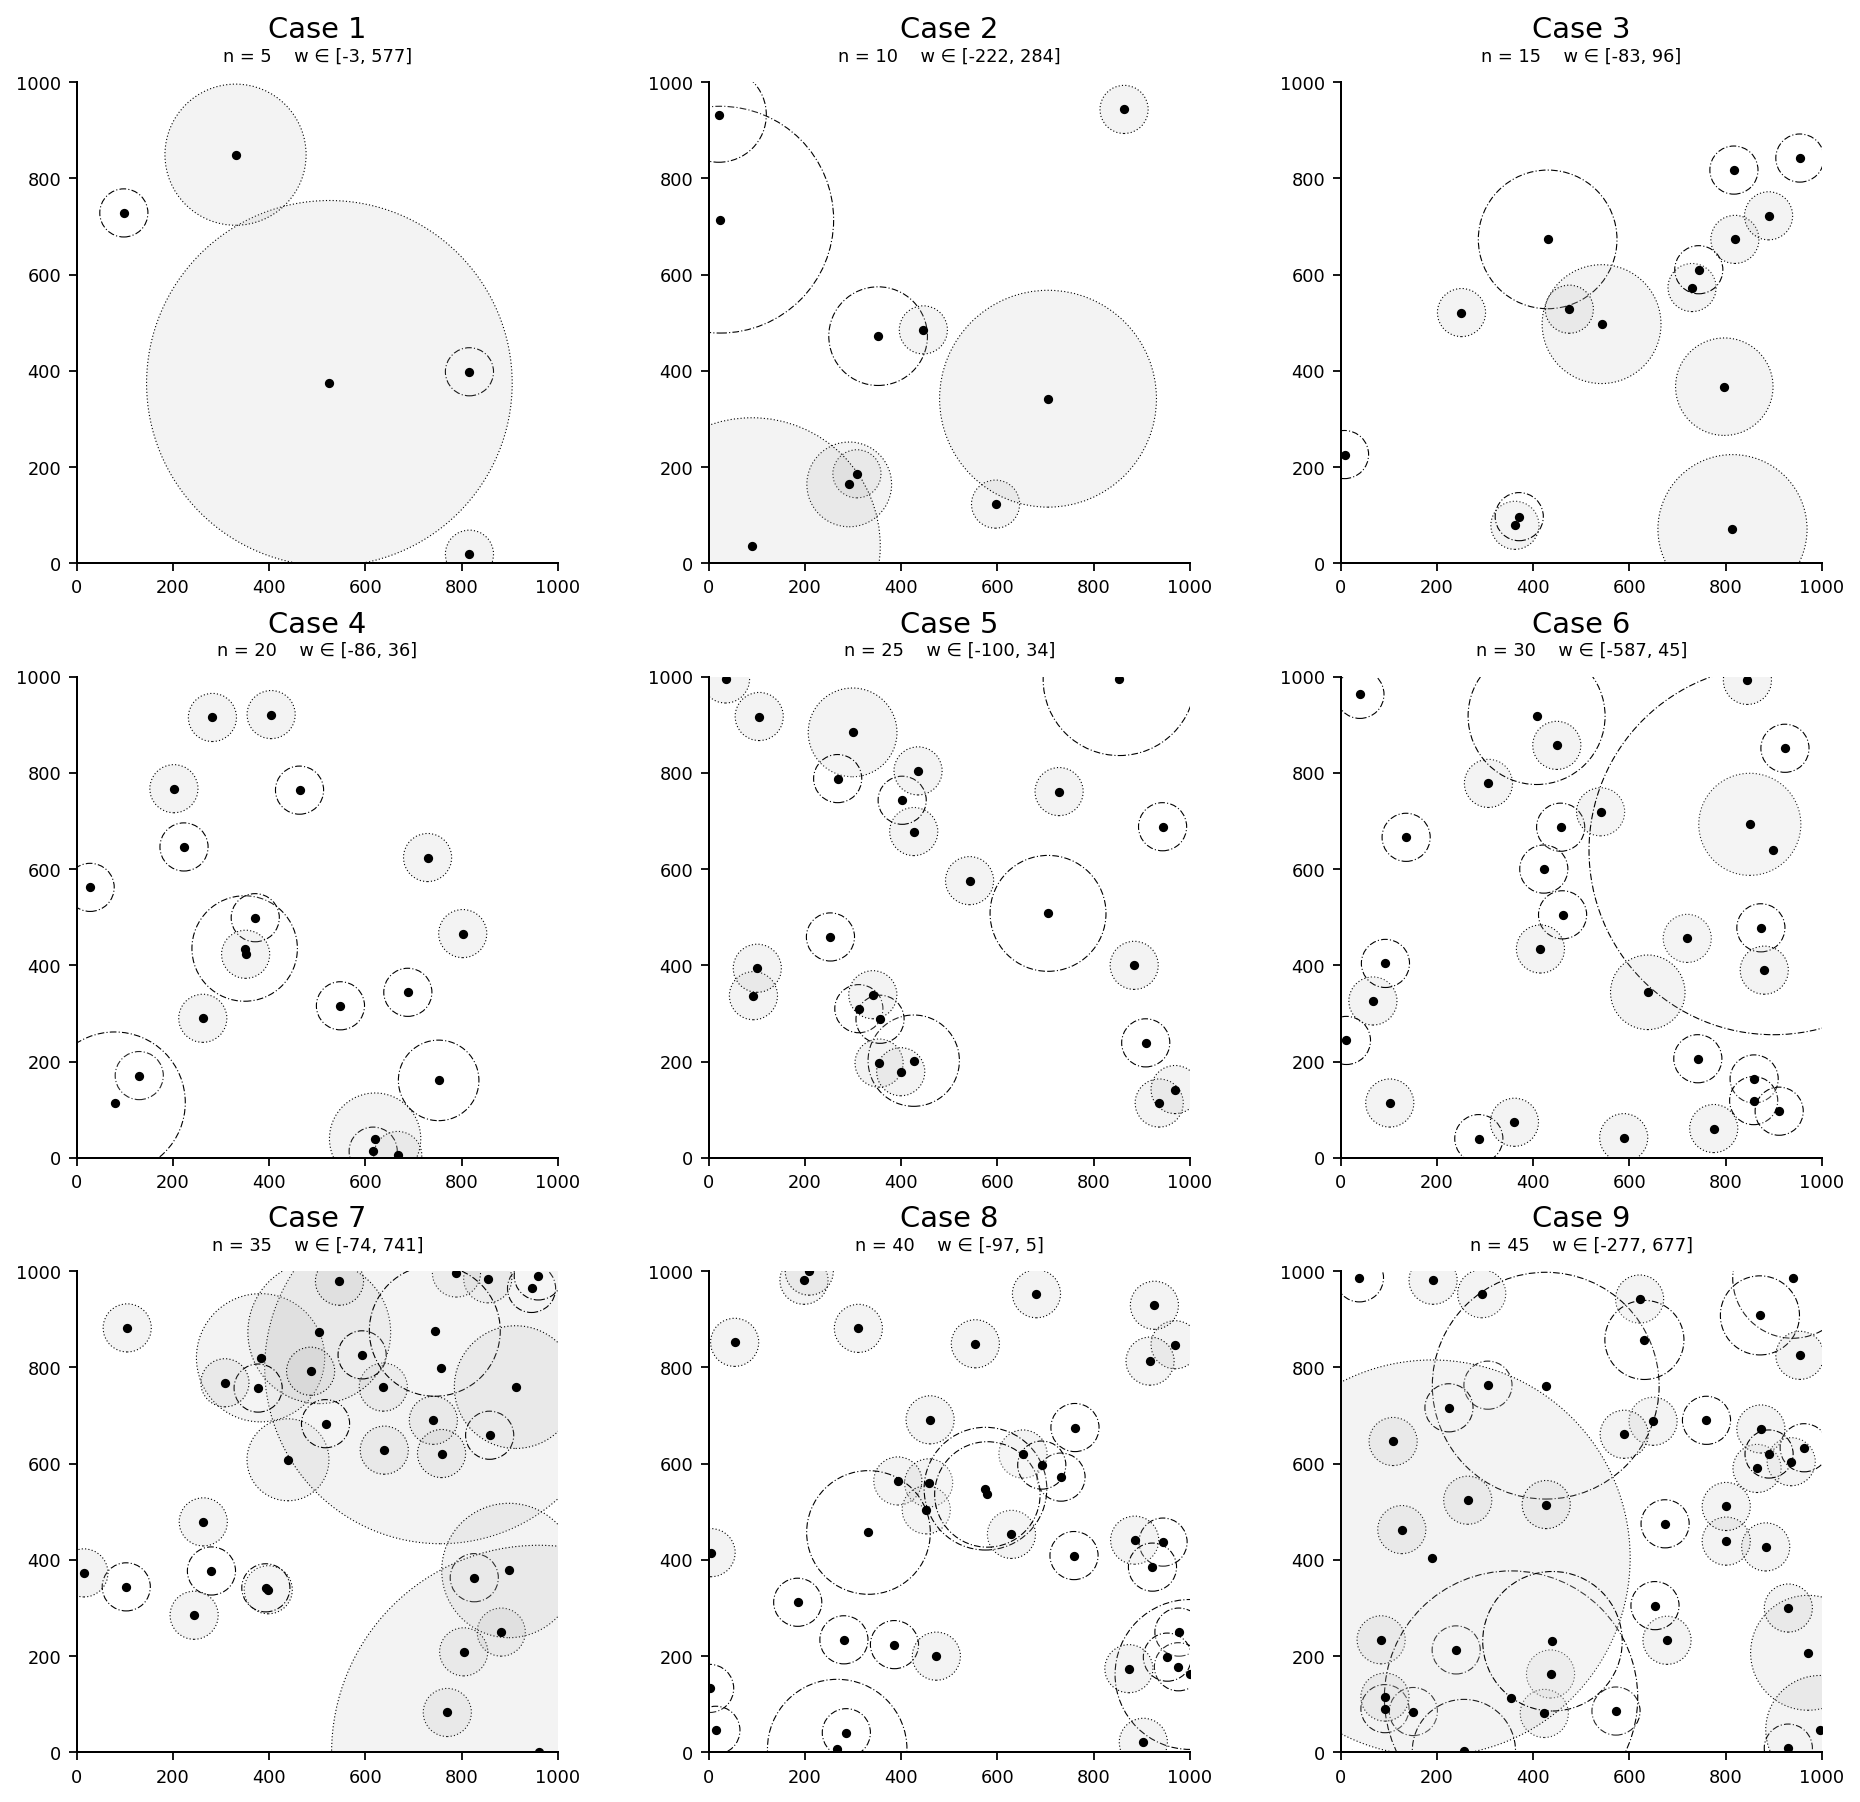
\includegraphics[width=0.95\linewidth]{Pictures/test_sites1.png}
    \caption{Generated weighted-site configurations for the first experiment ($n=5$ to $45$). 
    Each subfigure represents a distinct input size with randomized coordinates and weights within the displayed ranges.}
    \label{fig:test_sites1}
\end{figure}

\begin{figure}[H]
    \centering
    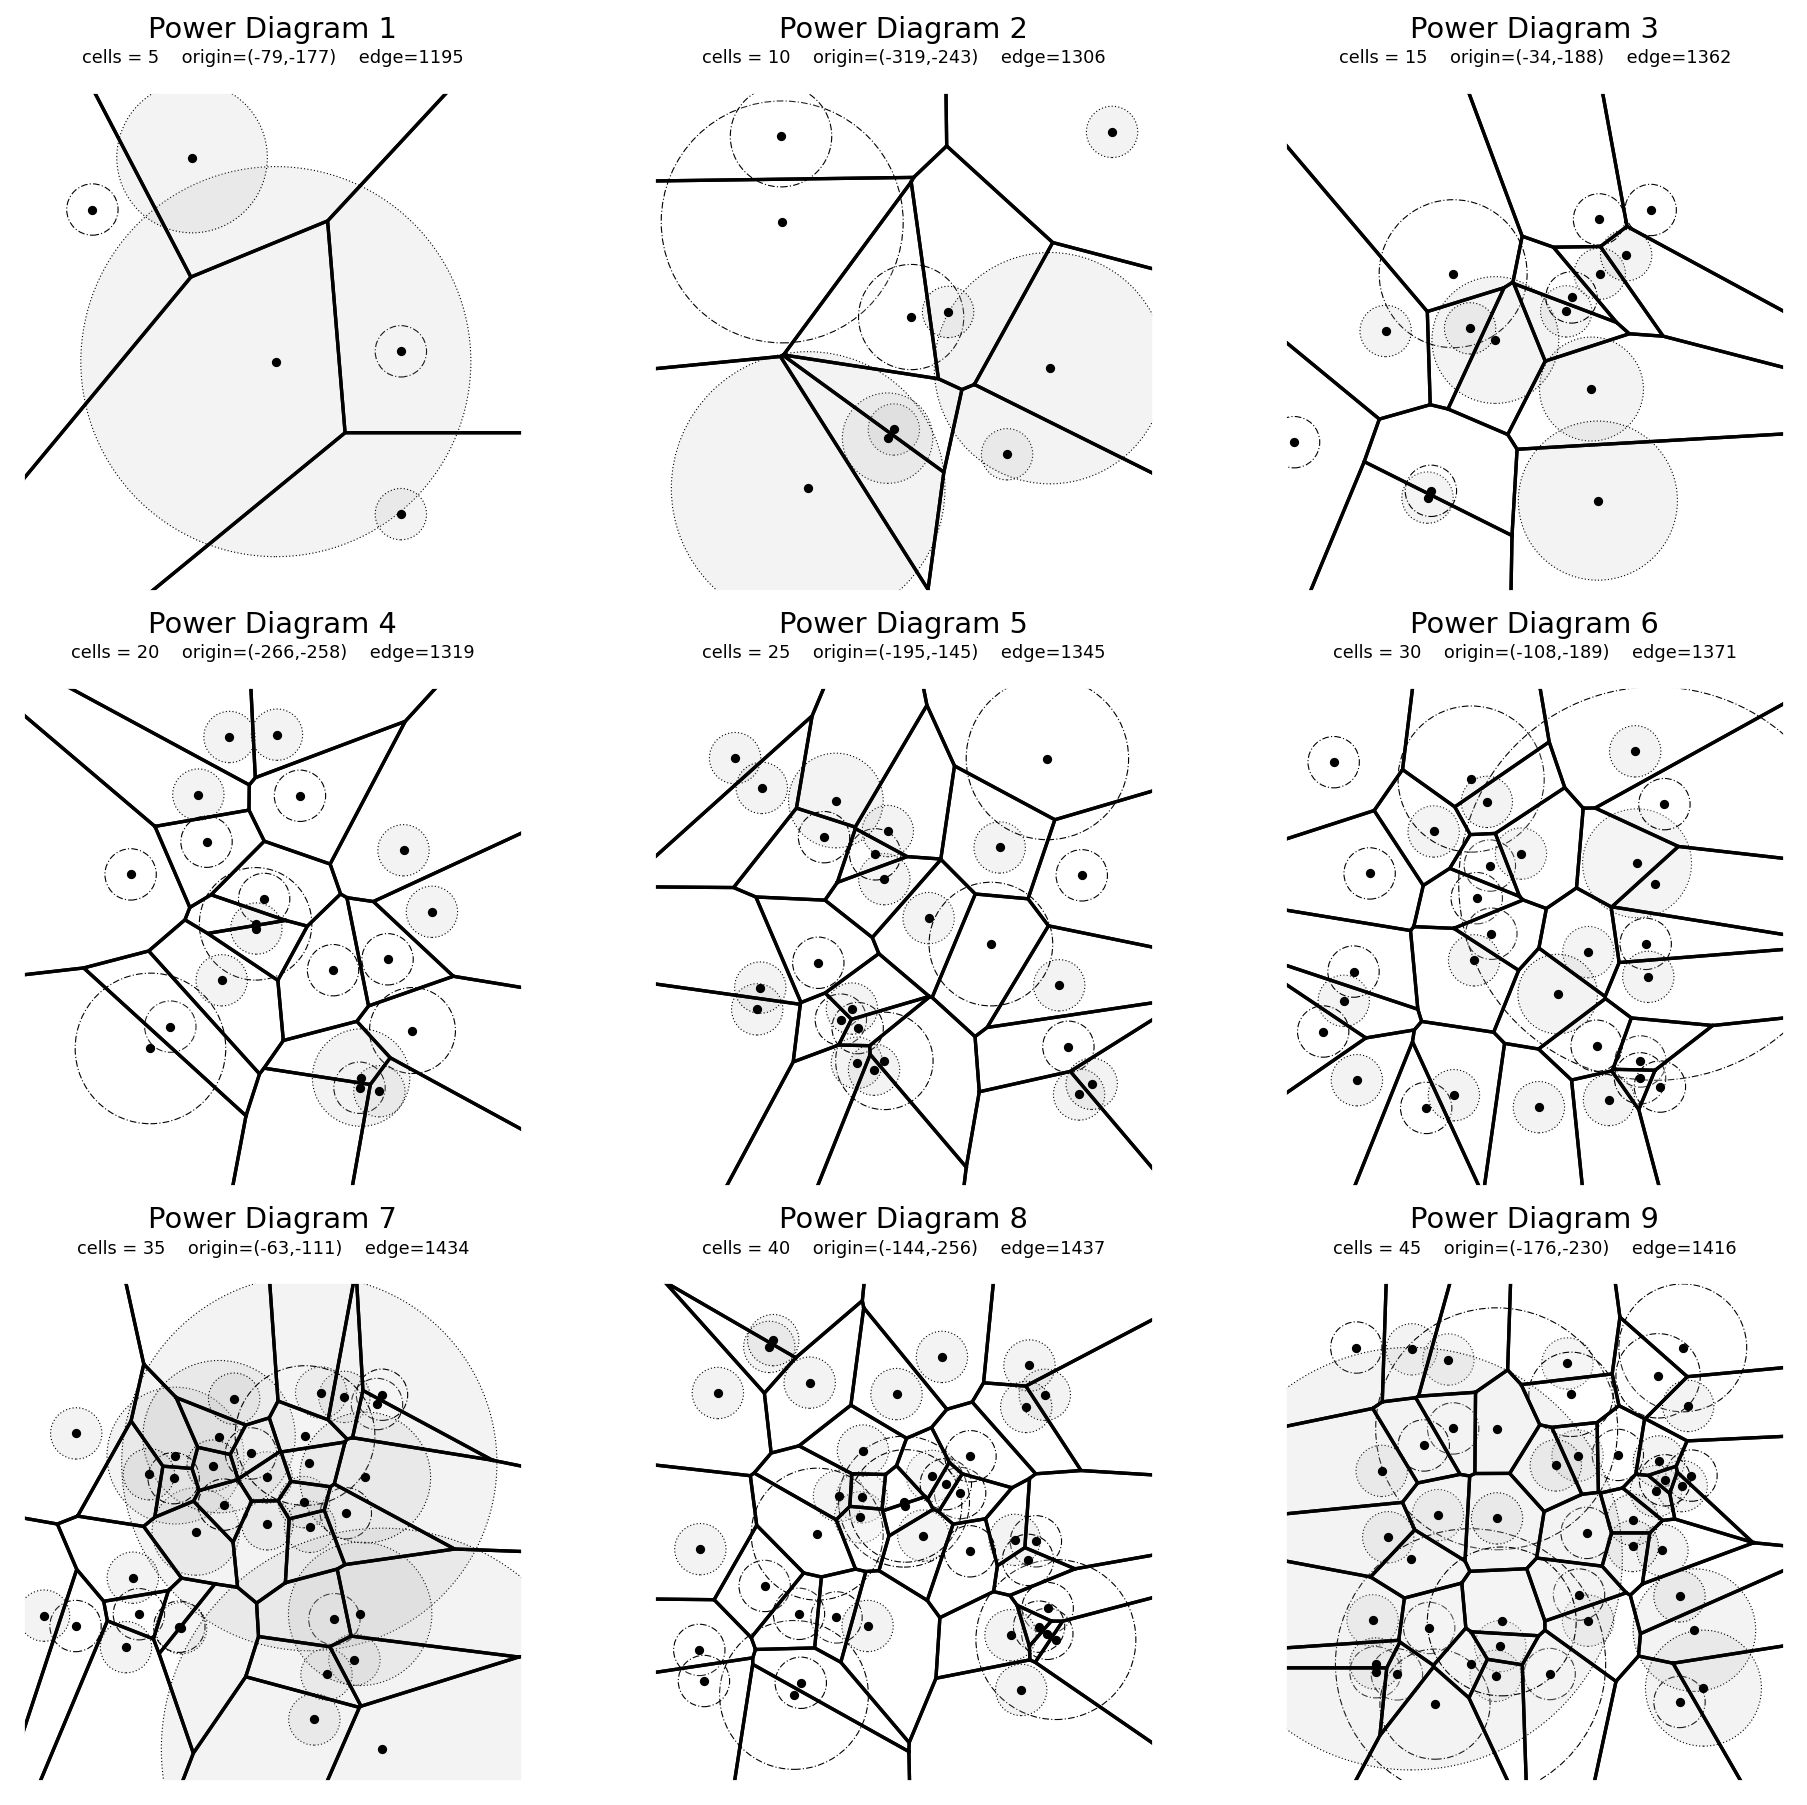
\includegraphics[width=0.95\linewidth]{Pictures/test_pd1.png}
    \caption{Resulting Power Diagrams corresponding to Figure~\ref{fig:test_sites1}. 
    Each diagram contains convex cells computed by half-plane intersections, with empty cells shown as unfilled regions.}
    \label{fig:test_pd1}
\end{figure}

\begin{figure}[H]
    \centering
    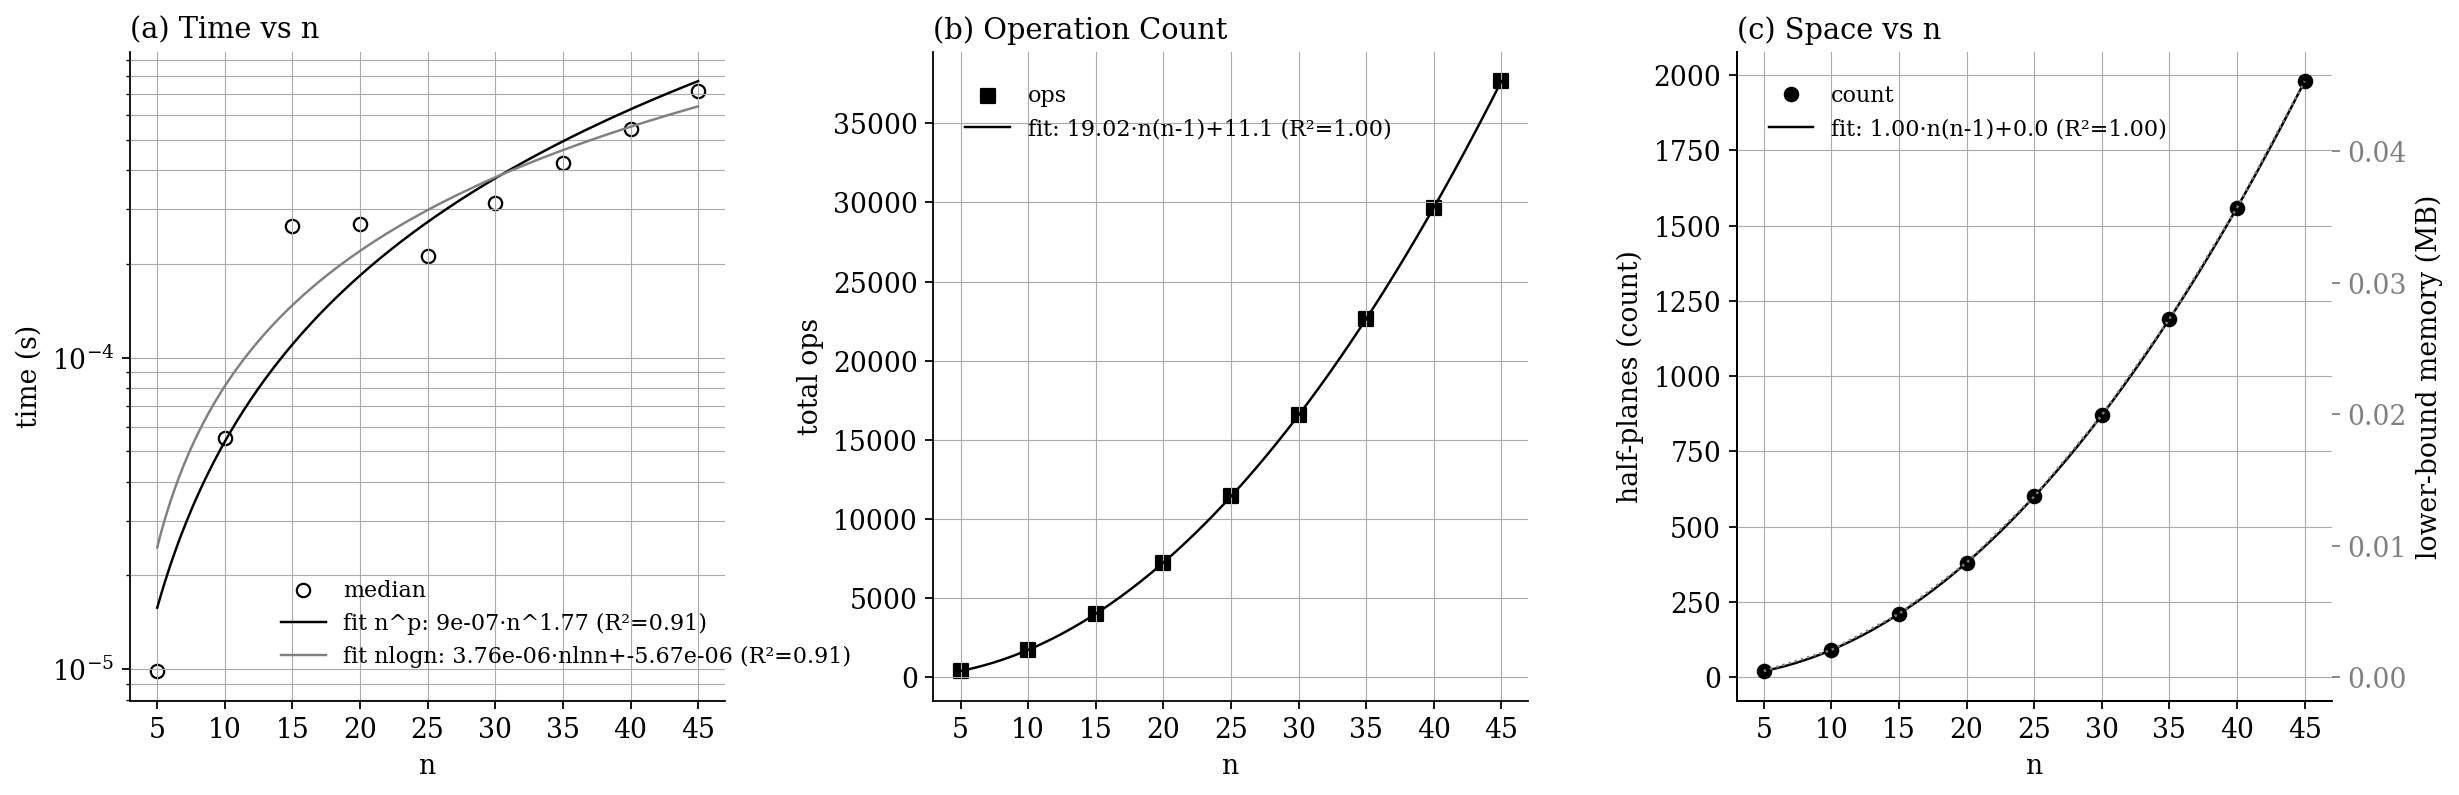
\includegraphics[width=0.95\linewidth]{Pictures/power_complexity1.png}
    \caption{Empirical complexity analysis for the first experiment ($n=5$–$45$). 
    (a) Median runtime vs.~$n$, fitted with power-law and $n\log n$ models; 
    (b) total operation count (half-plane computations) vs.~$n$, fitted with quadratic model; 
    (c) space cost vs.~$n$, showing stored half-plane growth and equivalent memory usage.}
    \label{fig:power_complexity1}
\end{figure}

\textbf{First-round observations:}
For smaller input sizes ($n\!\le\!45$), both the number of half-planes and total operation count follow a clear quadratic trend consistent with $\Theta(n^2)$ expectations.  
However, the runtime curve exhibits minor irregularities due to external factors such as system scheduling and interpreter-level overhead, which dominate at millisecond scales.  
The space cost remains perfectly quadratic with $R^2\!=\!1.00$, confirming that the number of stored half-planes grows as $n(n-1)$.

To mitigate runtime noise and strengthen asymptotic evidence, a second set of experiments extended the range up to $n=240$, improving fit quality for both time and operation scaling.

\begin{figure}[H]
    \centering
    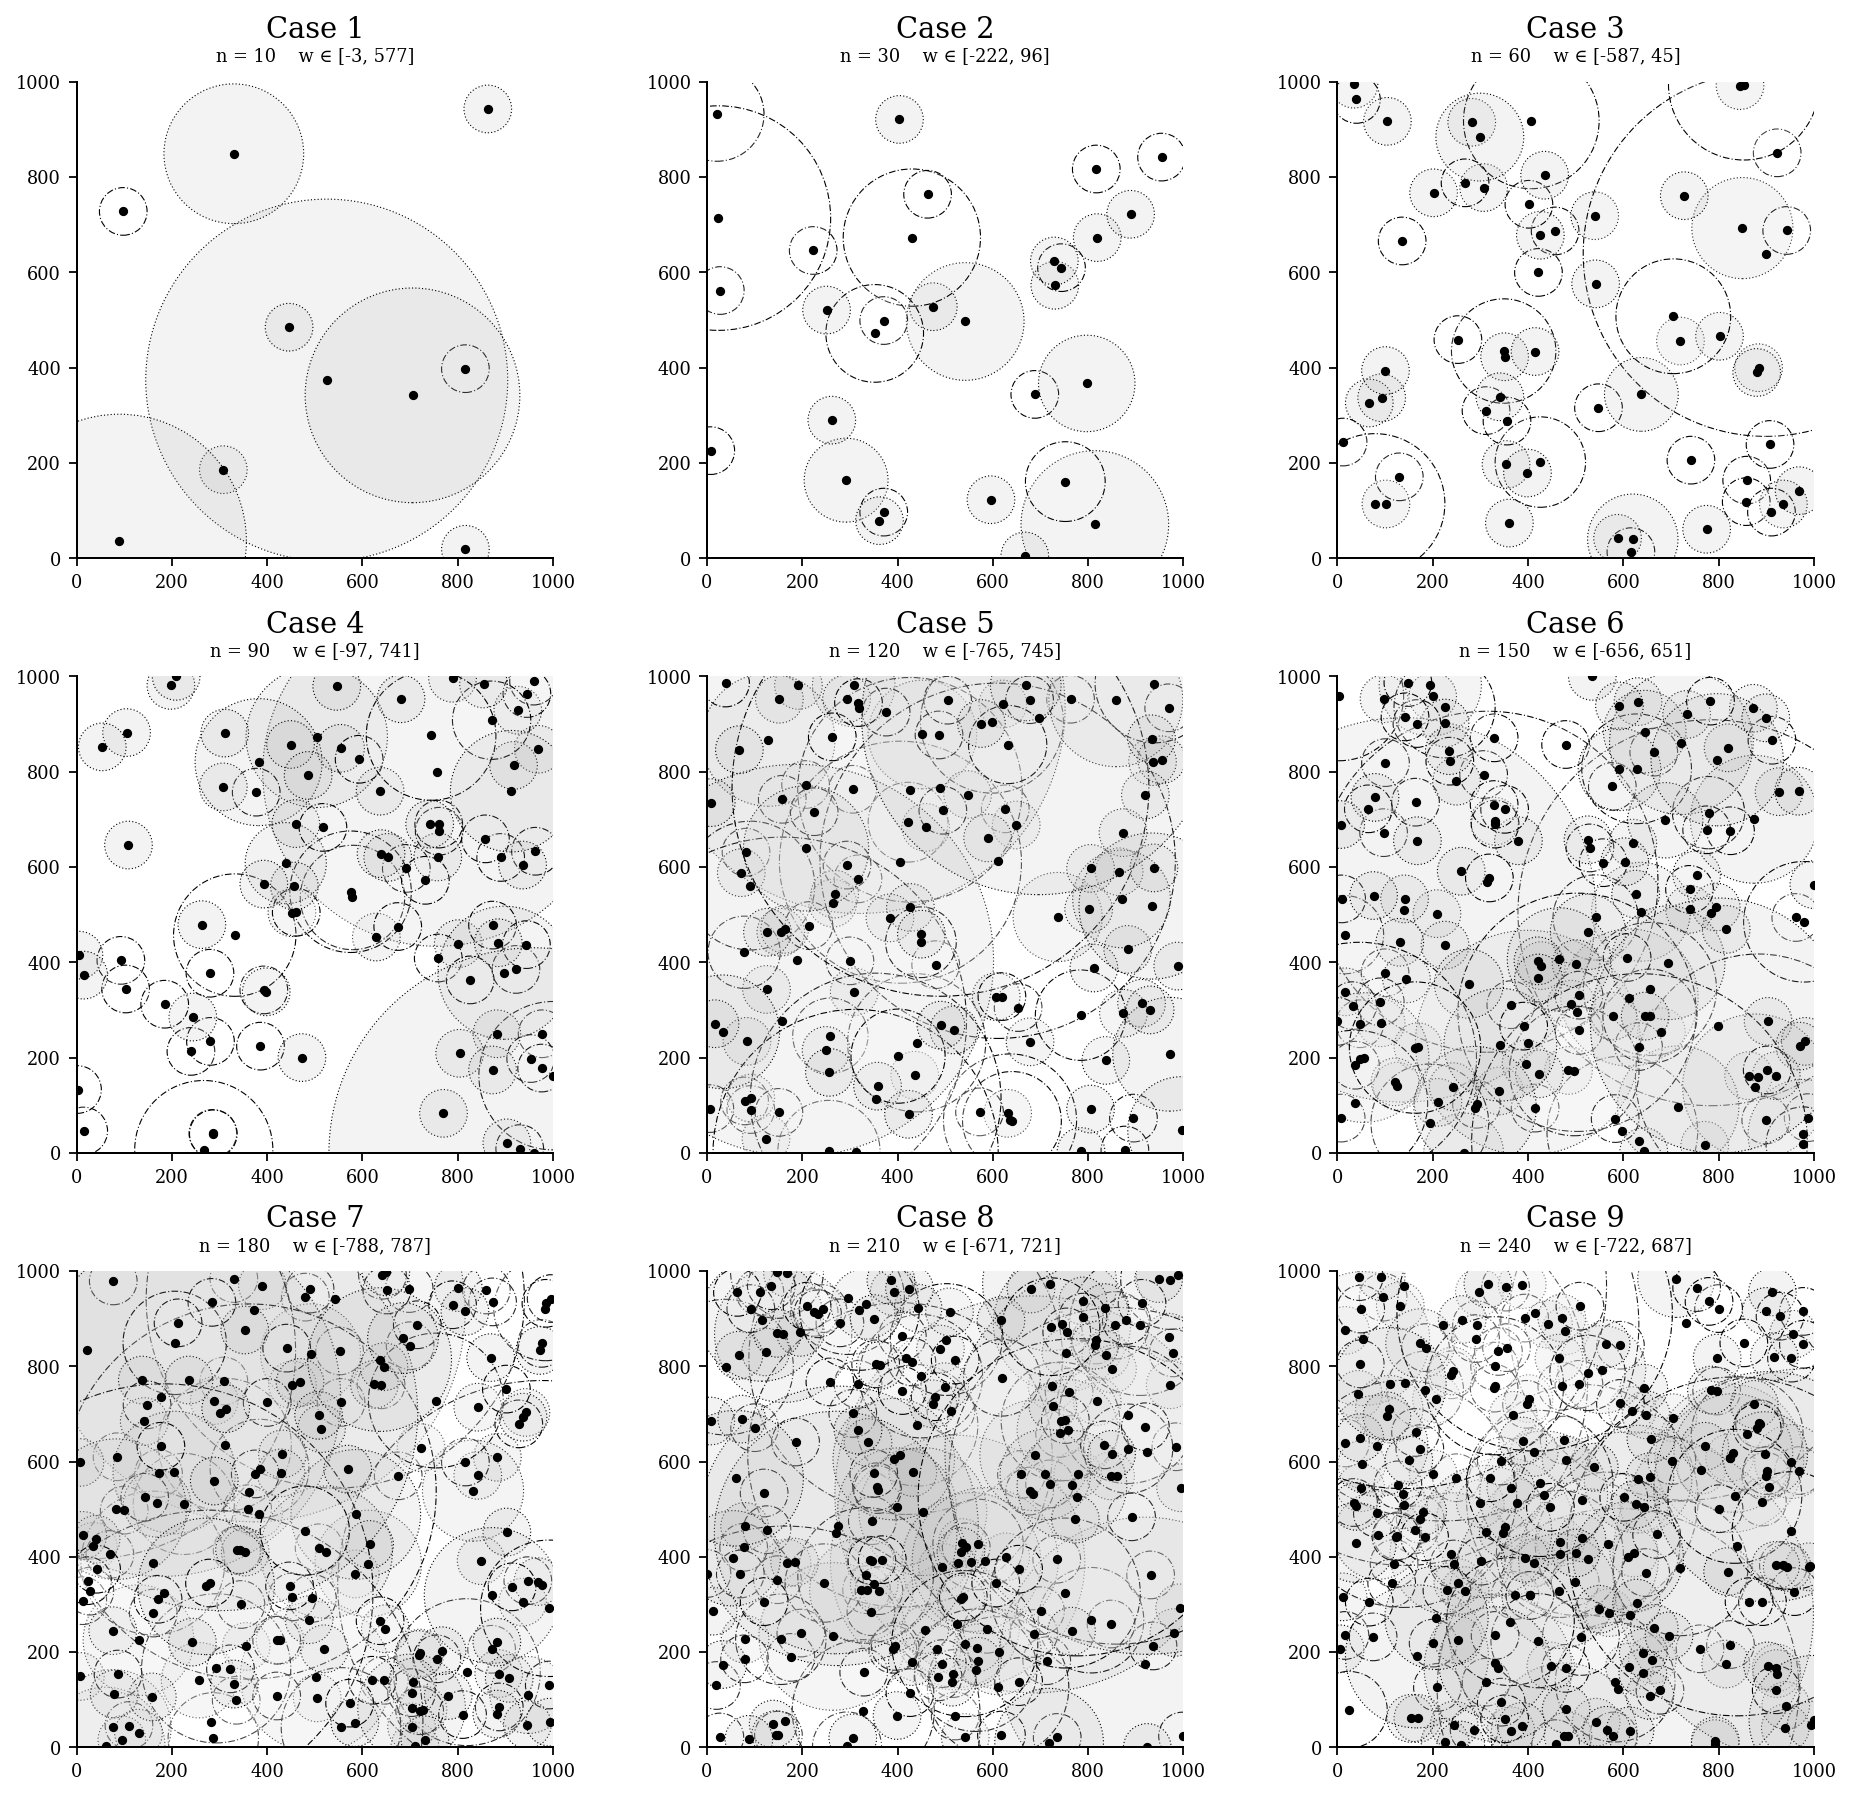
\includegraphics[width=0.95\linewidth]{Pictures/test_sites2.png}
    \caption{Weighted-site configurations for the second experiment ($n=10$ to $240$). 
    Larger sets ensure sufficient computational load to reveal true asymptotic behavior.}
    \label{fig:test_sites2}
\end{figure}

\begin{figure}[H]
    \centering
    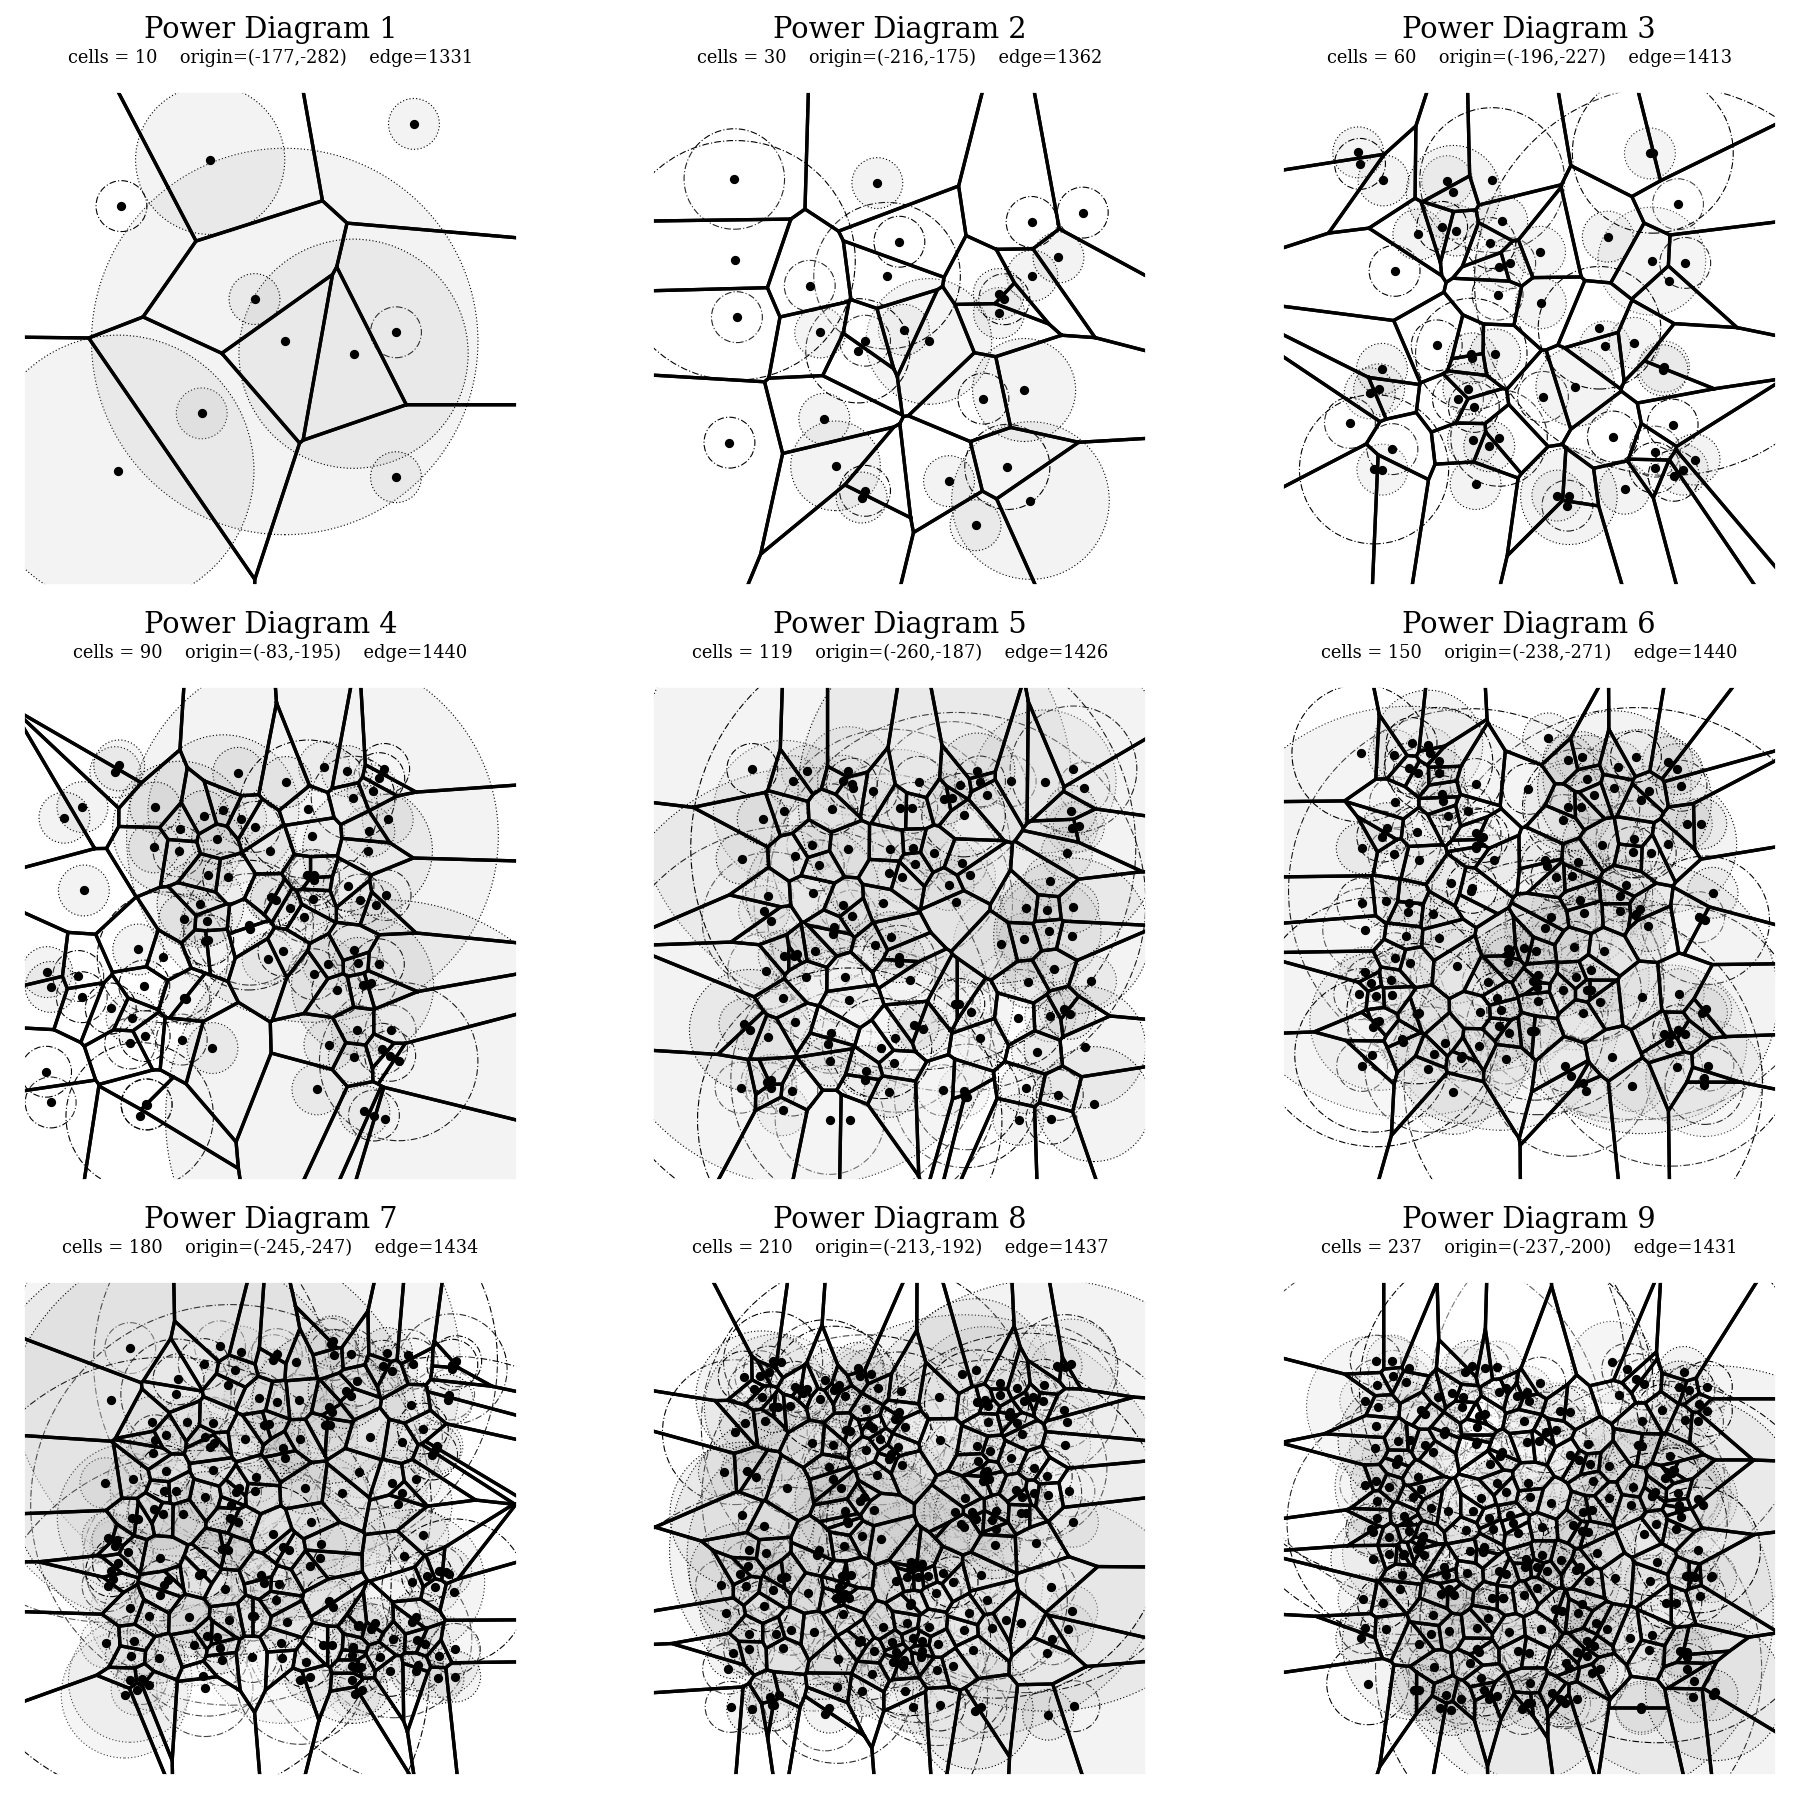
\includegraphics[width=0.95\linewidth]{Pictures/test_pd2.png}
    \caption{Power Diagrams corresponding to Figure~\ref{fig:test_sites2}. 
    Each subfigure shows correctly formed convex cells even at high densities, verifying numerical stability for large-scale inputs.}
    \label{fig:test_pd2}
\end{figure}

\begin{figure}[H]
    \centering
    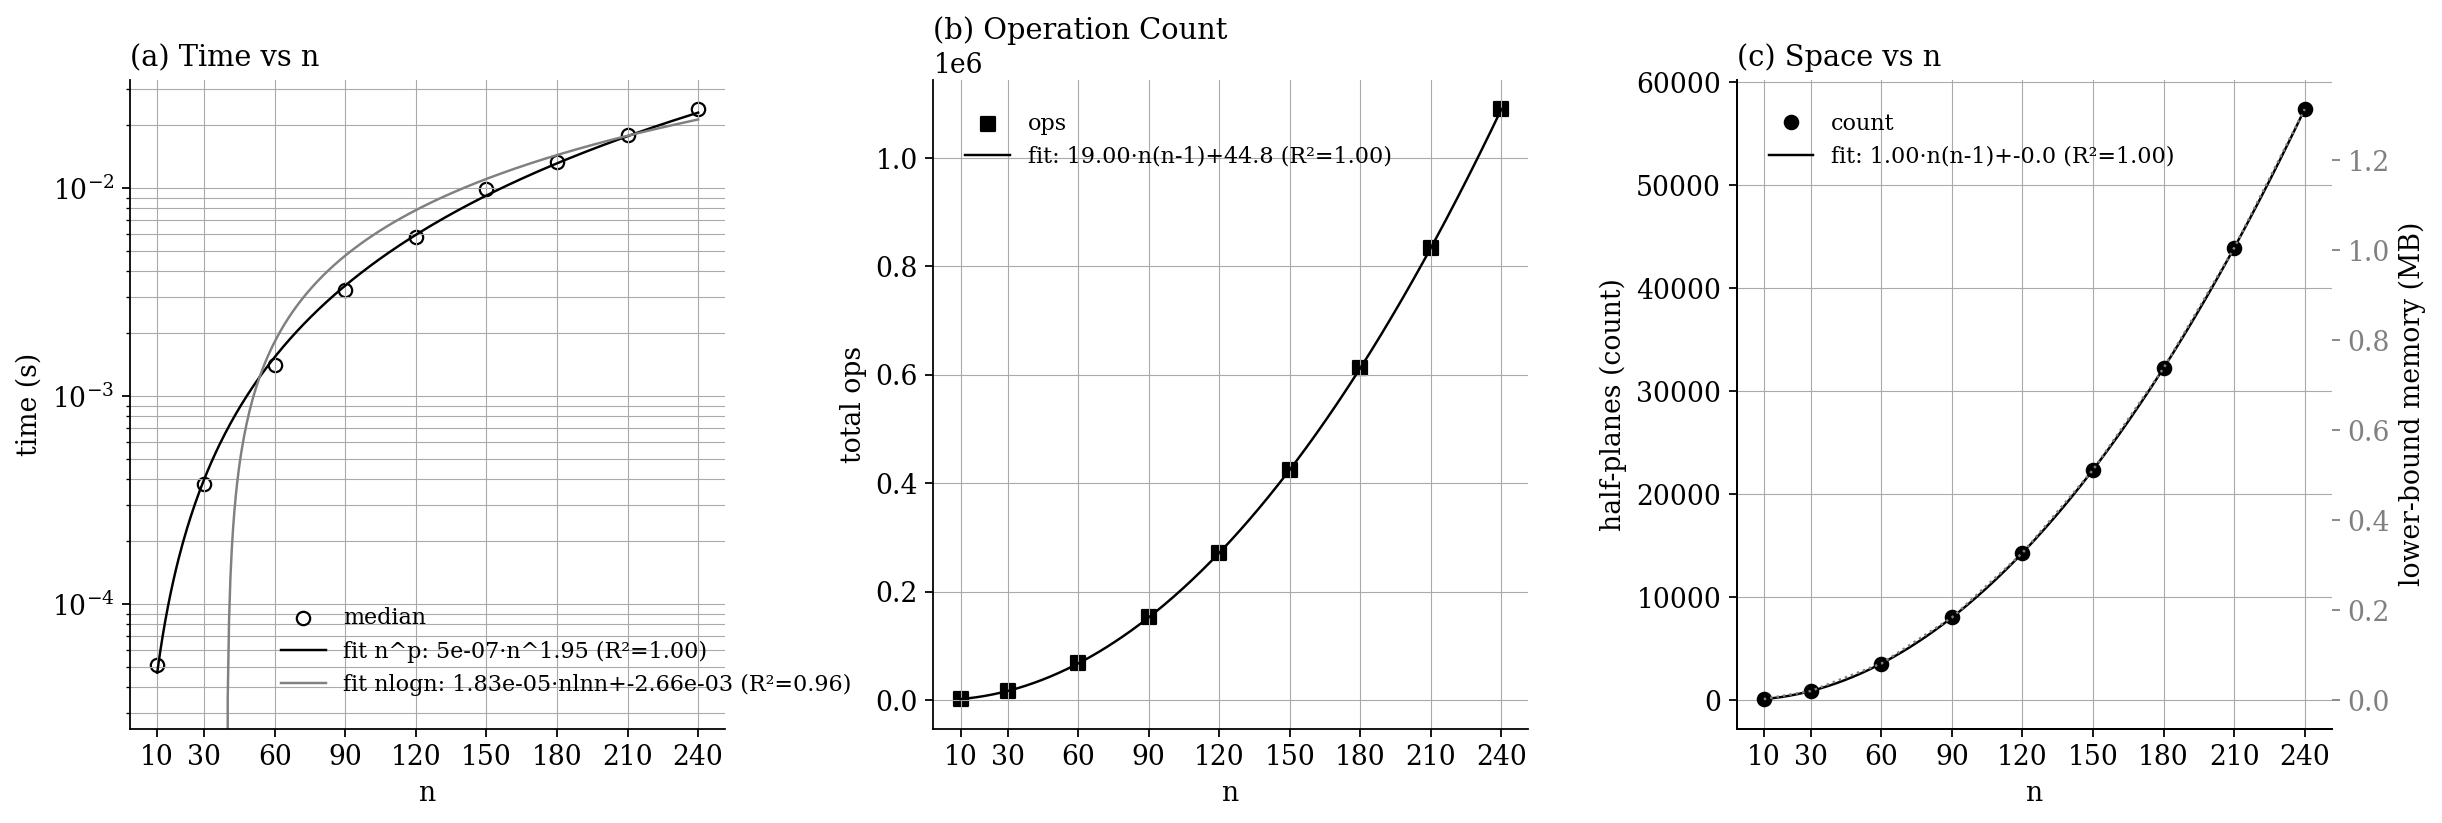
\includegraphics[width=0.95\linewidth]{Pictures/power_complexity2.png}
    \caption{Empirical complexity analysis for the second experiment ($n=10$–$240$). 
    (a) Median runtime fitted as $T(n)\propto n^{1.99}$ ($R^2=1.00$), closely matching the theoretical $\Theta(n^2)$ trend; 
    (b) total operation count fitted as $19.0\,n(n-1)+44.8$ ($R^2=1.00$); 
    (c) stored half-plane count and corresponding memory usage also showing perfect quadratic growth.}
    \label{fig:power_complexity2}
\end{figure}

\textbf{Discussion:}
Across both experimental rounds, the empirical results strongly corroborate the theoretical analysis.  
The total number of operations and stored half-planes follow an exact quadratic law with near-perfect coefficient of determination ($R^2\!\approx\!1.00$).  
The runtime scaling approaches $T(n)\!\propto\!n^{1.9\text{–}2.0}$, confirming the $\Theta(n^2)$ behavior once input sizes are sufficiently large to dominate constant and interpreter overheads.  
No deviations from convexity or numerical instability were observed even at $n=240$, demonstrating that the algorithm remains robust and predictable under large-scale weighted configurations.

Overall, the empirical evidence supports the theoretical conclusion that the implemented Power Diagram generator operates in $\Theta(n^2)$ time and $\Theta(n^2)$ space.  
The high-quality fits in both operation count and memory growth confirm that each site-to-site relation contributes a constant computational cost, validating the all-pairs bisector formulation and its deterministic complexity characteristics.

\newpage

\end{document}
